\documentclass[12pt, oneside]{article}

\usepackage{texmf/preamble}
\usepackage{texmf/macros}
\usepackage{texmf/wordcount}

\graphicspath{{./assets/}}
\addglobalbib{sources.bib}


\begin{document} % BEGIN

\pagenumbering{gobble}
\begin{titlepage}
    \large

    \begin{center}

        \vspace*{2cm}

        {\bfseries
            IB Math Analysis and Approaches (HL) \\
            Extended Essay\\
            May 2024 Session}\\

        \vspace*{\fill}

        \rule{\linewidth}{1.5pt} \\ [0.5cm]
        {\LARGE \bfseries The Mathematics Techniques of Camera Calibration}
        \rule{\linewidth}{0.5pt} \\

        \vspace*{\fill}

        \textbf{Research Question:} What are the various strategies and mathematical techniques employed in camera calibration to develop precise and accurate camera models?\\ [1cm]

        \textbf{Word Count:} \wordcount words

        \vspace*{2cm}

    \end{center}

\end{titlepage}

% =========================
\pagestyle{frontmatter}
\pagenumbering{roman}
\tableofcontents

% =========================
\clearpage
\pagestyle{mainmatter}
\pagenumbering{arabic}

\section{Introduction}

3D reconstruction from multiple images is the process of generating an accurate 3D model of a physical object from its 2D images. The process employs techniques from the broader science of photogrammetry, which is concerned with obtaining precise measurements of 3-dimensional physical objects from photographic images. The use of photogrammetry as a method of 3D reconstruction was first employed by Prussian architect Albrecht Meydenbauer in the 1860s, who created some of the earliest topographic plans and elevations drawings realized using photogrammetric techniques \autocite{ices2017}. Today, photogrammetry has applications in a wide variety of fields, including but not limited to: architecture, engineering, forensics, medicine, and geology.

\subsection{Overview of 3D Reconstruction}



The task of generating an accurate 3D model from various 2D images is a multi-step process, and consists of:




and they mainly fall into two main categories. The first method is based on the cross-referencing of keypoints between the images. Computer algorithms such as SIFT (Scale Invariant Feature Transform) and SURF (Speeded-Up Robust Features)

projective geometry to triangulate the position of keypoints of the objects. These keypoints are cross-referenced between the images either by hand or using a computer algorithm, and then


Camera calibration is a important








\section{Approach} 

There are many techniques one could take to calibrate a camera, 




\subsection{Camera Model} \label{sec:camera_model}

A camera model is a projection model which approximates the function of a camera by describing a mathematical relationship between points in 3D space and its projection onto the sensor grid of the camera. In order to construct such a model, we must first understand the general workings of a camera.

The modern lens camera is highly sophisticated, built with an array of complex mechanisms and a wide range of features such as zoom and autofocus. However, we only need to focus on its three principal elements critical to image projection: the lens, the aperture, and the sensor grid (CCD). 

\begin{itemize}[leftmargin=!, itemindent=-5ex]
    \item \textbf{Lens} -- Focuses incoming light rays and projects it onto the sensor grid. Modern cameras have compound lenses (lenses made up of several lens elements) in order to minimize undesired effects such as aberration, blurriness, and distortion. 
    \item \textbf{Aperture} -- Controls the amount of light that reaches the sensor. By adjusting the aperture size, the exposure and depth of field can be modified.
    \item \textbf{Sensor Grid} -- Captures incoming light rays and converts this information into pixels on an image. 
\end{itemize}

\begin{figure}[H]
    \centering
    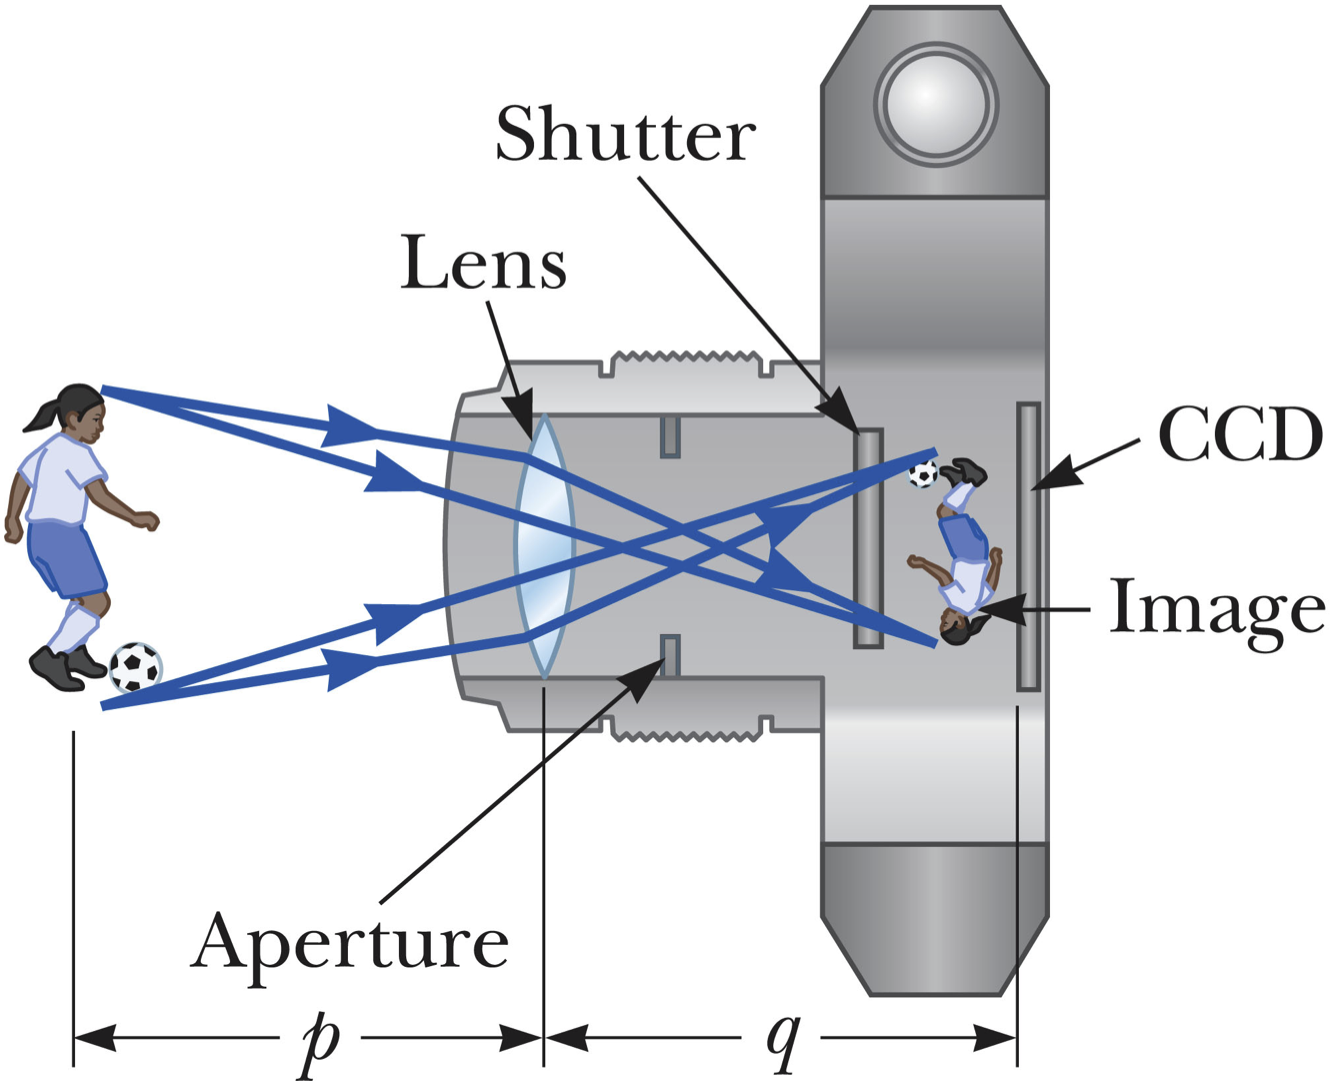
\includegraphics[width=0.5\textwidth]{images/lens_camera}
    \caption{Lens camera. Adapted from \cite{coltonPhysics1232012}} \label{fig:lens_camera}
\end{figure}

However, it is impossible to construct a model which is both simple and exact for the lens cameras, as the behavior of lenses are very complex. As such, it is mathematically convenient to approximate the camera as a pinhole camera. In doing so, we ignore lens distortion, but it distills the behavior of a camera to its most fundamental and essential dynamics: the projection of points in 3D space onto the flat 2D image plane. 

\subsubsection{Pinhole Camera Model}

A pinhole camera is a simple camera without a lens. It instead relies on the use of a tiny hole as the aperture of the camera, and light rays pass through the hole, projecting an inverted image onto the image plane. The pinhole camera model is based on the pinhole camera, however it goes further by making the assumption that the aperture is infinitely small. This means that any incoming light ray would only travel in straight lines, going through the pinhole mapping to one singular point on the image plane. 

\begin{figure}[H]
    \centering
    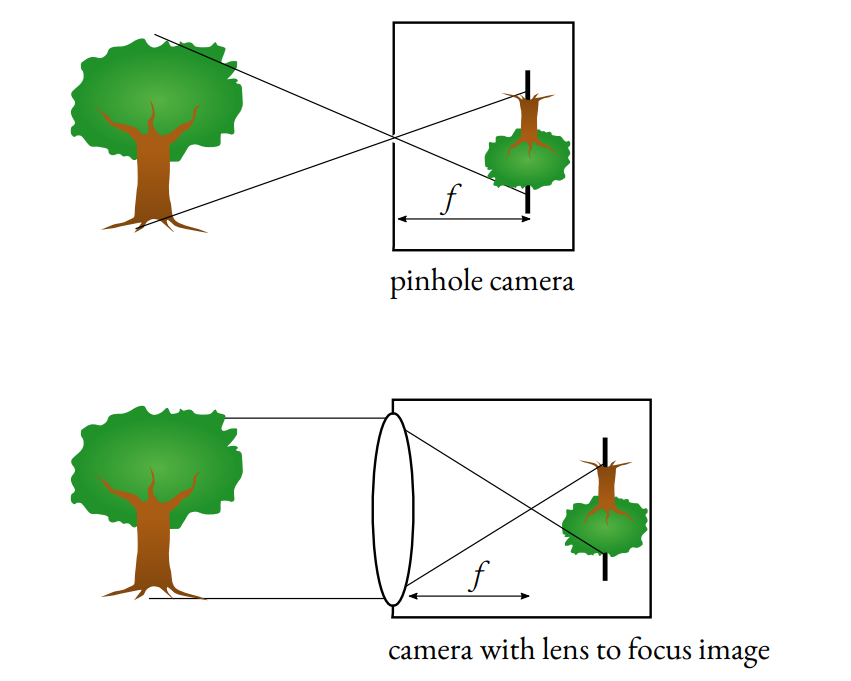
\includegraphics[width=0.7\textwidth]{images/pinhole_vs_lens}
    \caption{Difference between a pinhole camera and a lens camera. Adapted from \cite{leCameraModel2018}}
\end{figure}

If necessary, one could reintroduce distortion and shear terms in order to minimize the error, but this is often not needed for low to medium precision applications, as the distortion of modern lenses are already minimal. As such, its ease of use has led it to become one of the most frequently employed camera models in the field of camera calibration. 

\subsection{Calibration Object}

The calibration object is an object with known dimensions and features which is often used in camera calibration to 


Calibration objects can be constructed in many ways, and they can be separated into different categories based the dimension of the calibration object \footcite{zhangCameraCalibration2007}.

\begin{itemize}[leftmargin=!, itemindent=-4ex]
    \item \textbf{3D object based calibration} -- Performed by using a calibration object whose geometry is known to very high precision. Typically, the calibration object consists of 2 or 3 orthogonal planes, although a plane whose precise translation is known may also be used, which also yields 3D reference points \footcite{zhangCameraCalibration2007}. Using 3D objects is typically preferred, as it yields the highest accuracy \footcite{zhangCameraCalibration2007}, and the mathematics required is also the least. 
    \item \textbf{2D plane-based calibration} -- The most common technique is known as Zhang's method, and it requires a planar object (often a checkerboard pattern), and various pictures of this plane are taken at different orientations \footcite{zhangFlexibleNew2000}. Knowledge of the translation of the plane is not necessary. Due to its easier setup and good accuracy, it is the best choice in most situations. In fact, the most commonly used camera vision programming library, \texttt{OpenCV}, is geared towards this type of calibration. 
    \item \textbf{1D line-based calibration} -- Typically requires analyzing more than three photographs with straight lines which are not parallel with each other \footcite{chuLineBasedCamera2005}. 
\end{itemize}

One can also calibrate cameras without a calibration object, using featuring tracking of objects in the scene to estimate camera parameters. This process is often referred to as self-calibration or auto-calibration. However, this is less preferable, as it involves a lot of estimation of parameters, which not only means that it is a more mathematically complex problem, it may not be able to achieve the accuracy of calibration using known calibration patterns \footcite{zhangCameraCalibration2007}. As such, it is typically the only chosen when pre-calibration is impossible. 

For this paper, I will focus on calibration using a 3D calibration object, because the mathematics behind it is simpler, and many of the techniques used in 3D-based calibration are 

\section{Constructing the Pinhole Camera Model}

\begin{figure}[H]
    \centering
    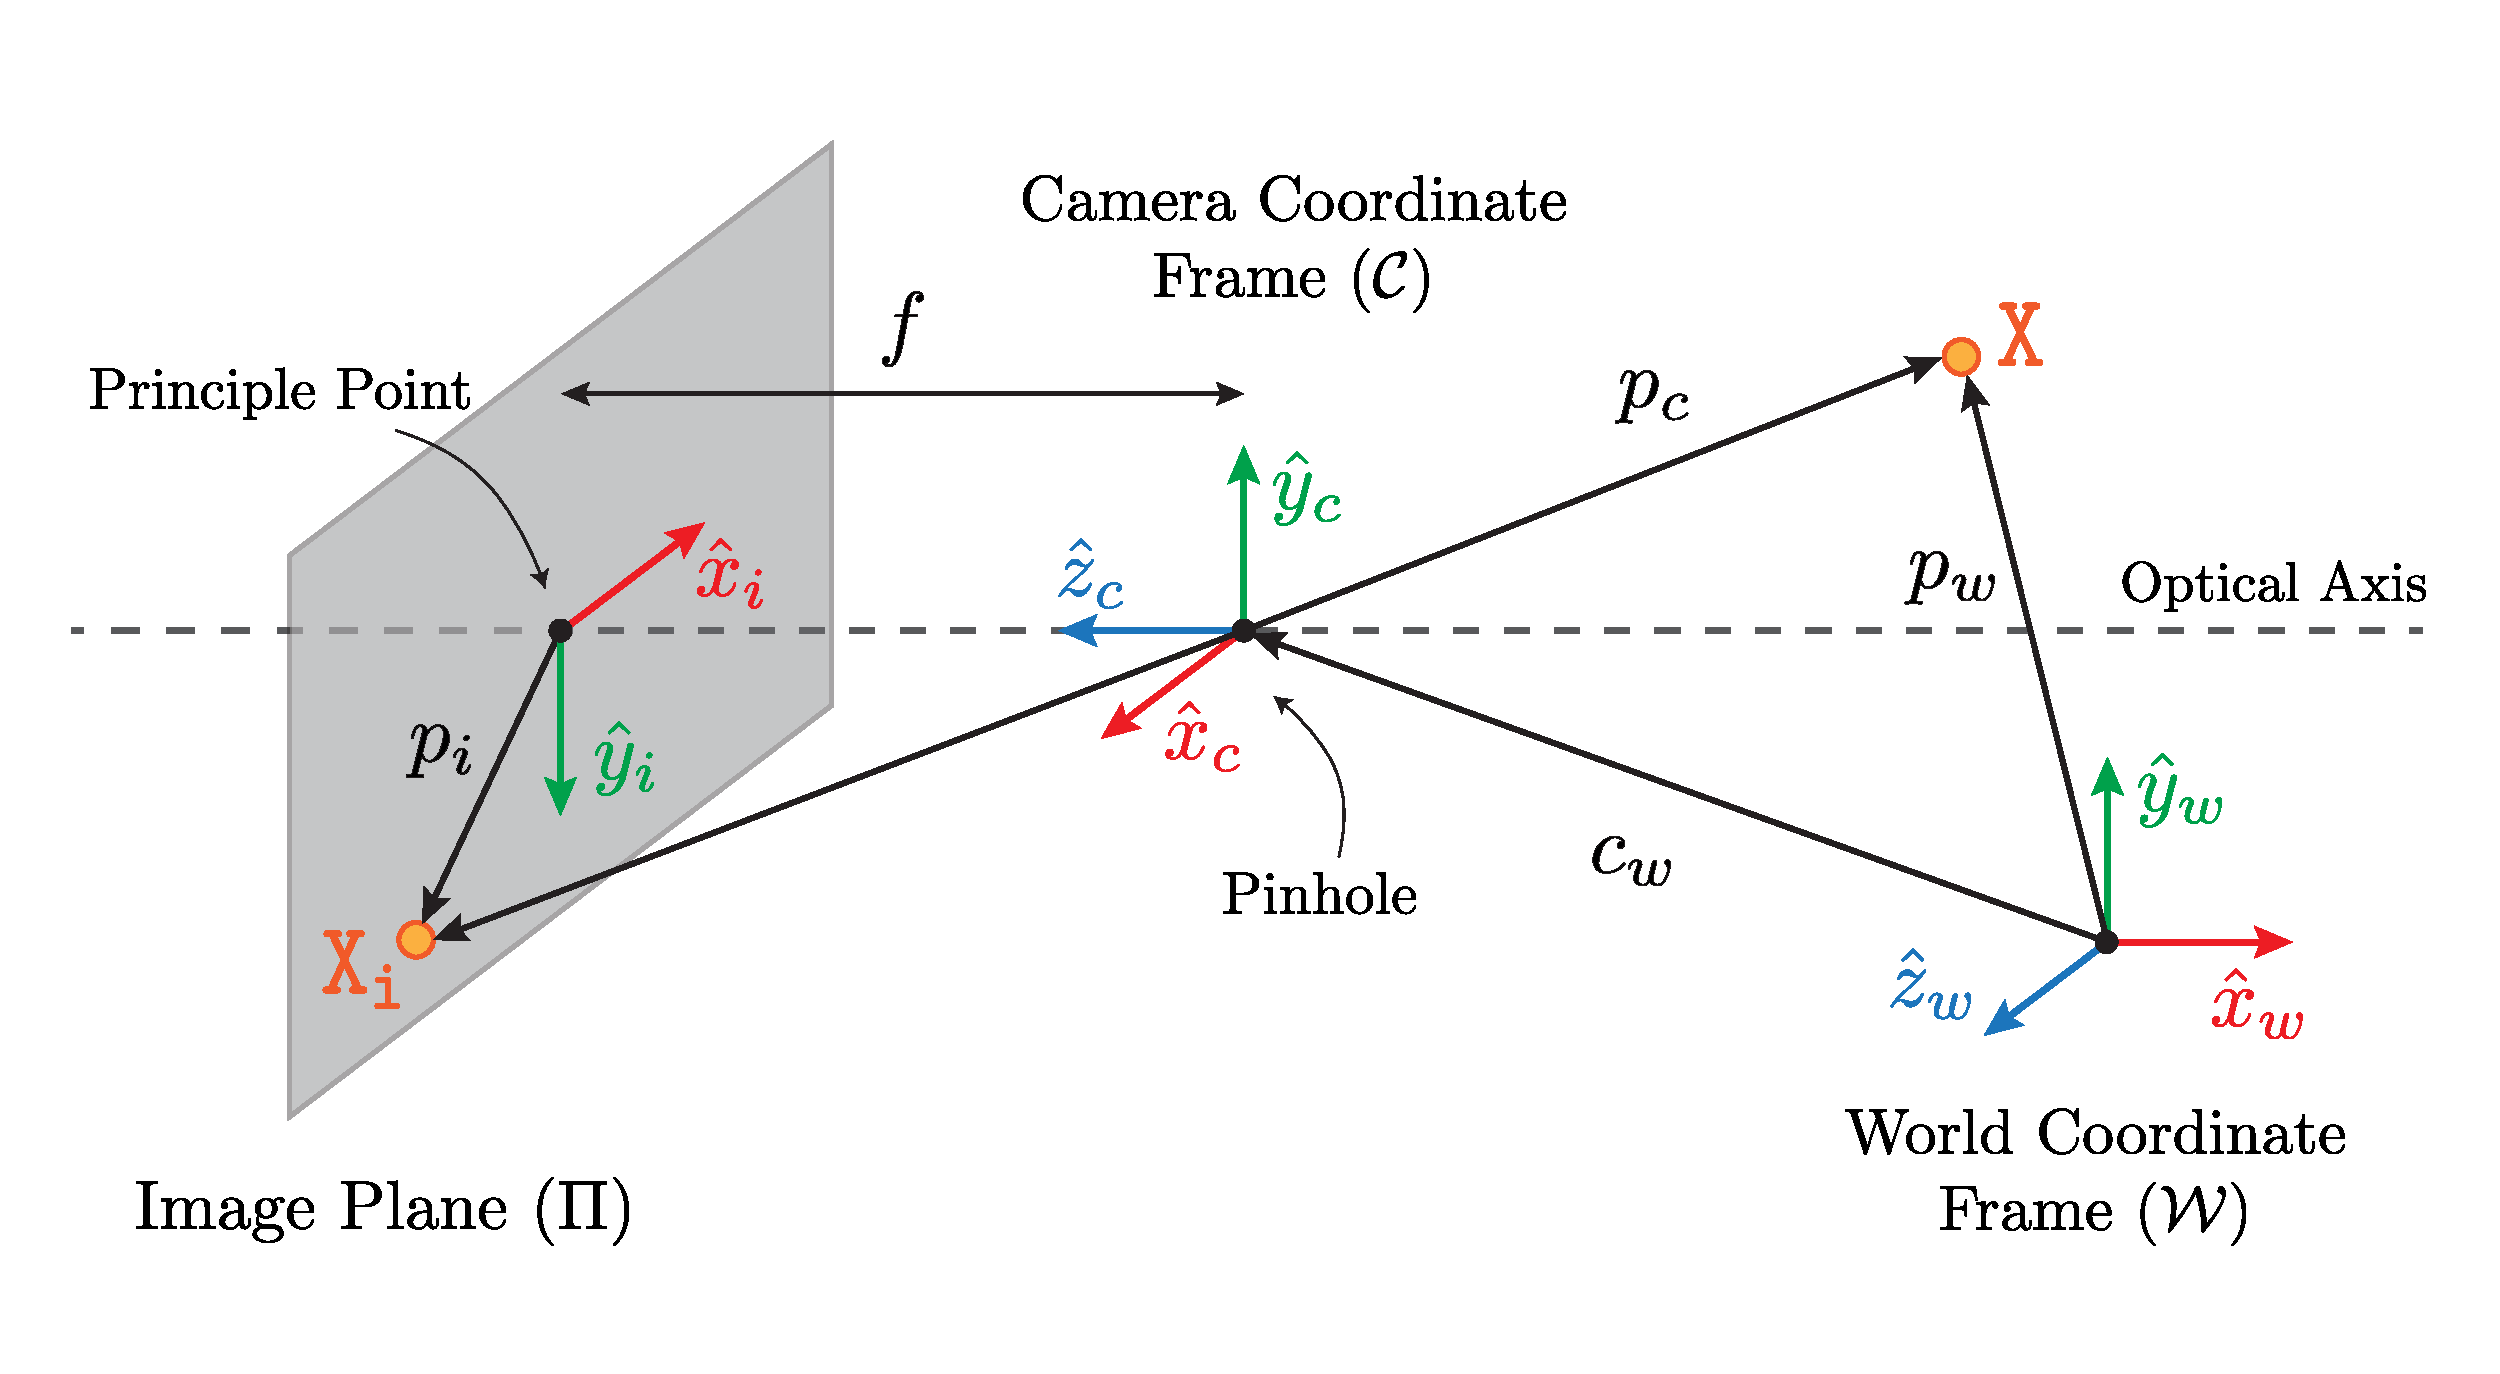
\includegraphics[width=0.9\textwidth]{diagrams/imaging_model}
    \caption{Pinhole camera model.}
\end{figure}

The construction of the pinhole camera model involves defining the relationships between the 3D world, the pinhole camera, and the resulting 2D image. To reflect these  4 different frames of reference, all of which :
\begin{itemize}[leftmargin=!, itemindent=-4ex]
    \item\textbf{World Coordinate Frame ($\boldsymbol{\mathcal{W}}$)}. Represents the 3D space of the scene being photographed, with respect to an origin which may be arbitrary and depends on the conventions chosen. Objects that are in the scene are defined with respect to this coordinate frame.
    \item\textbf{Camera Coordinate Frame ($\boldsymbol{\mathcal{C}}$)}. Represents the 3D space of the scene being photographed, but with respect to the pinhole (aperture) of the camera.
    \item\textbf{Image Coordinate Frame ($\boldsymbol{\Pi}$)}. 2D plane representing the image sensor plane of the camera. The origin is the principle point of the image sensor, where the optical axis intersects the image plane.
    \item\textbf{Pixel Coordinate Frame}. 2D plane representing the position of pixels on the image sensor. The discrete version of the image coordinate frame, where c
\end{itemize}

The optical axis of a camera is an imaginary line which passes through the center of the aperture of the camera.



\begin{figure}[H]
    \centering
    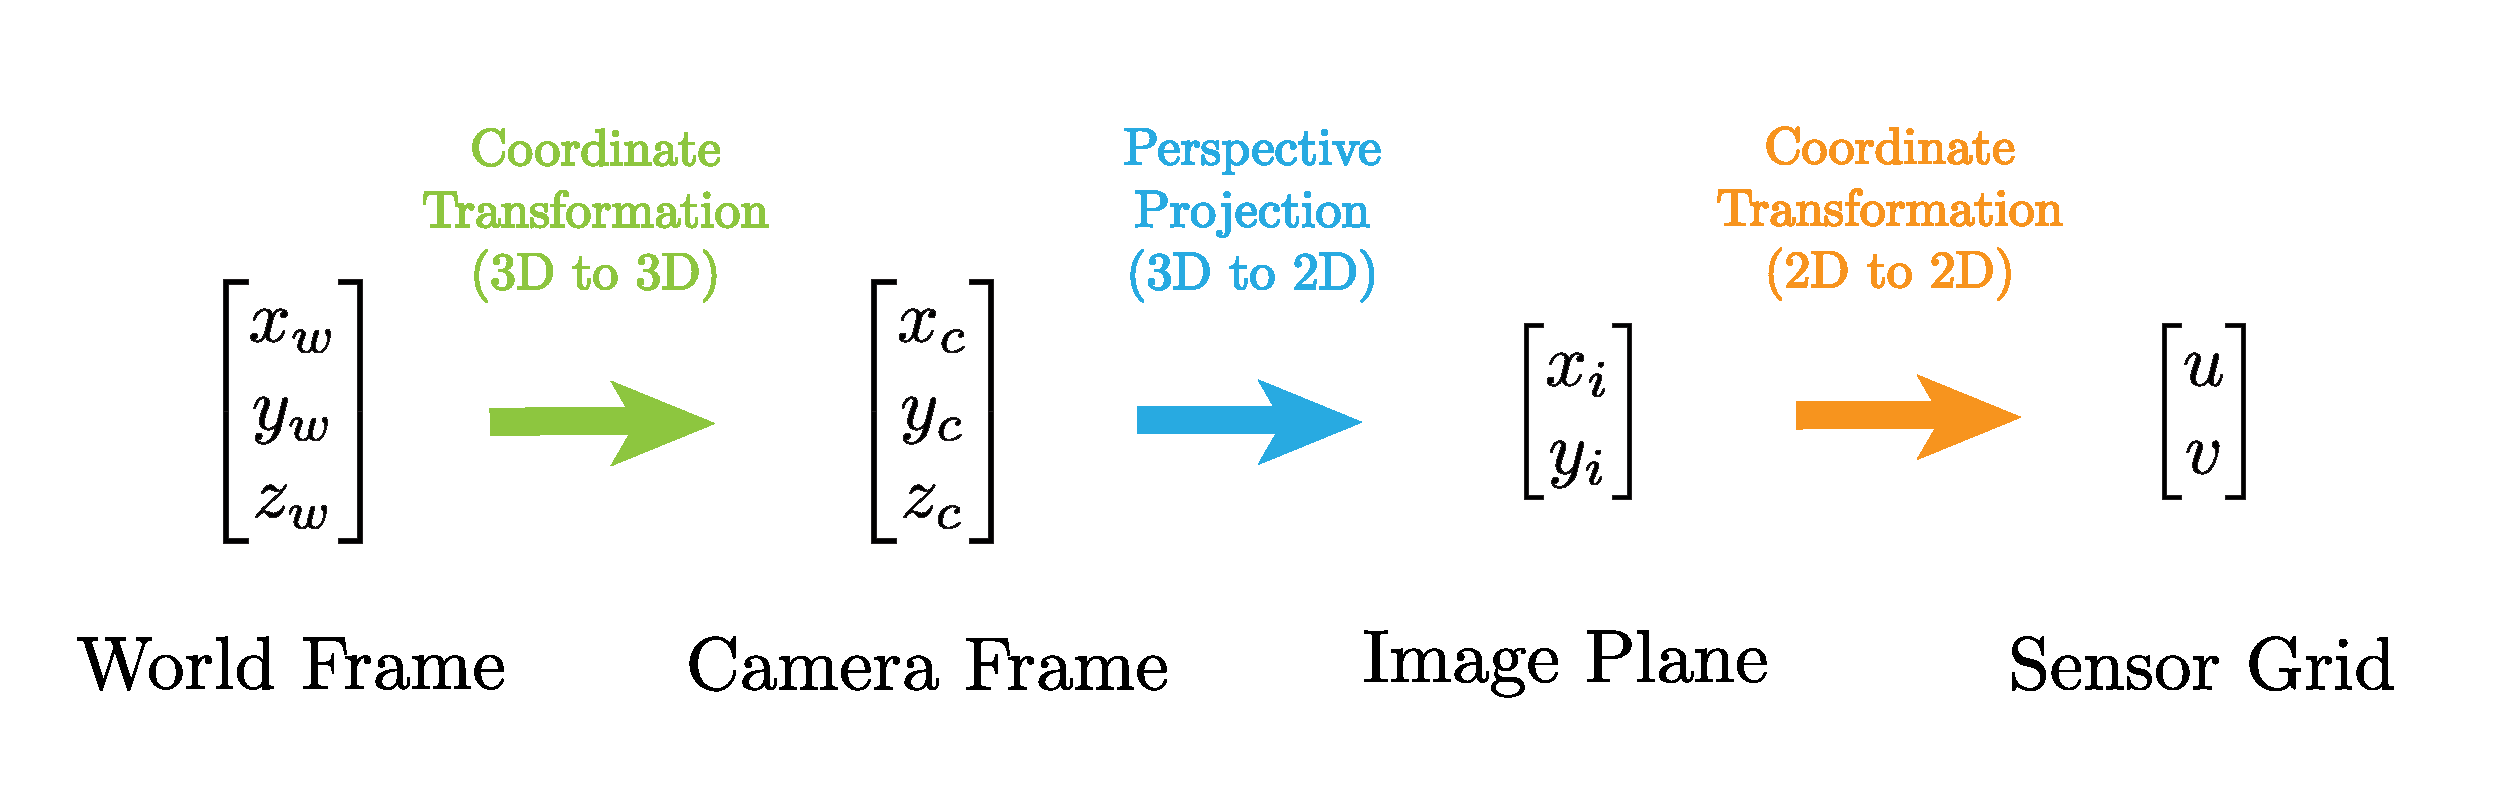
\includegraphics[width=0.9\textwidth]{diagrams/coord_conversions}
    \caption{Coordinate transformations.}
\end{figure}


\subsection{Intrinsic Parameters} \label{sec:intrinsics}

Intrinsic parameters describe the internal characteristics of the camera. In other words, it dictates how in the 3D space are projected onto the image plane, i.e. the relationship between the position of the point $\mathtt{X}$ to its projection on the image plane.

\begin{figure}[H]
    \centering
    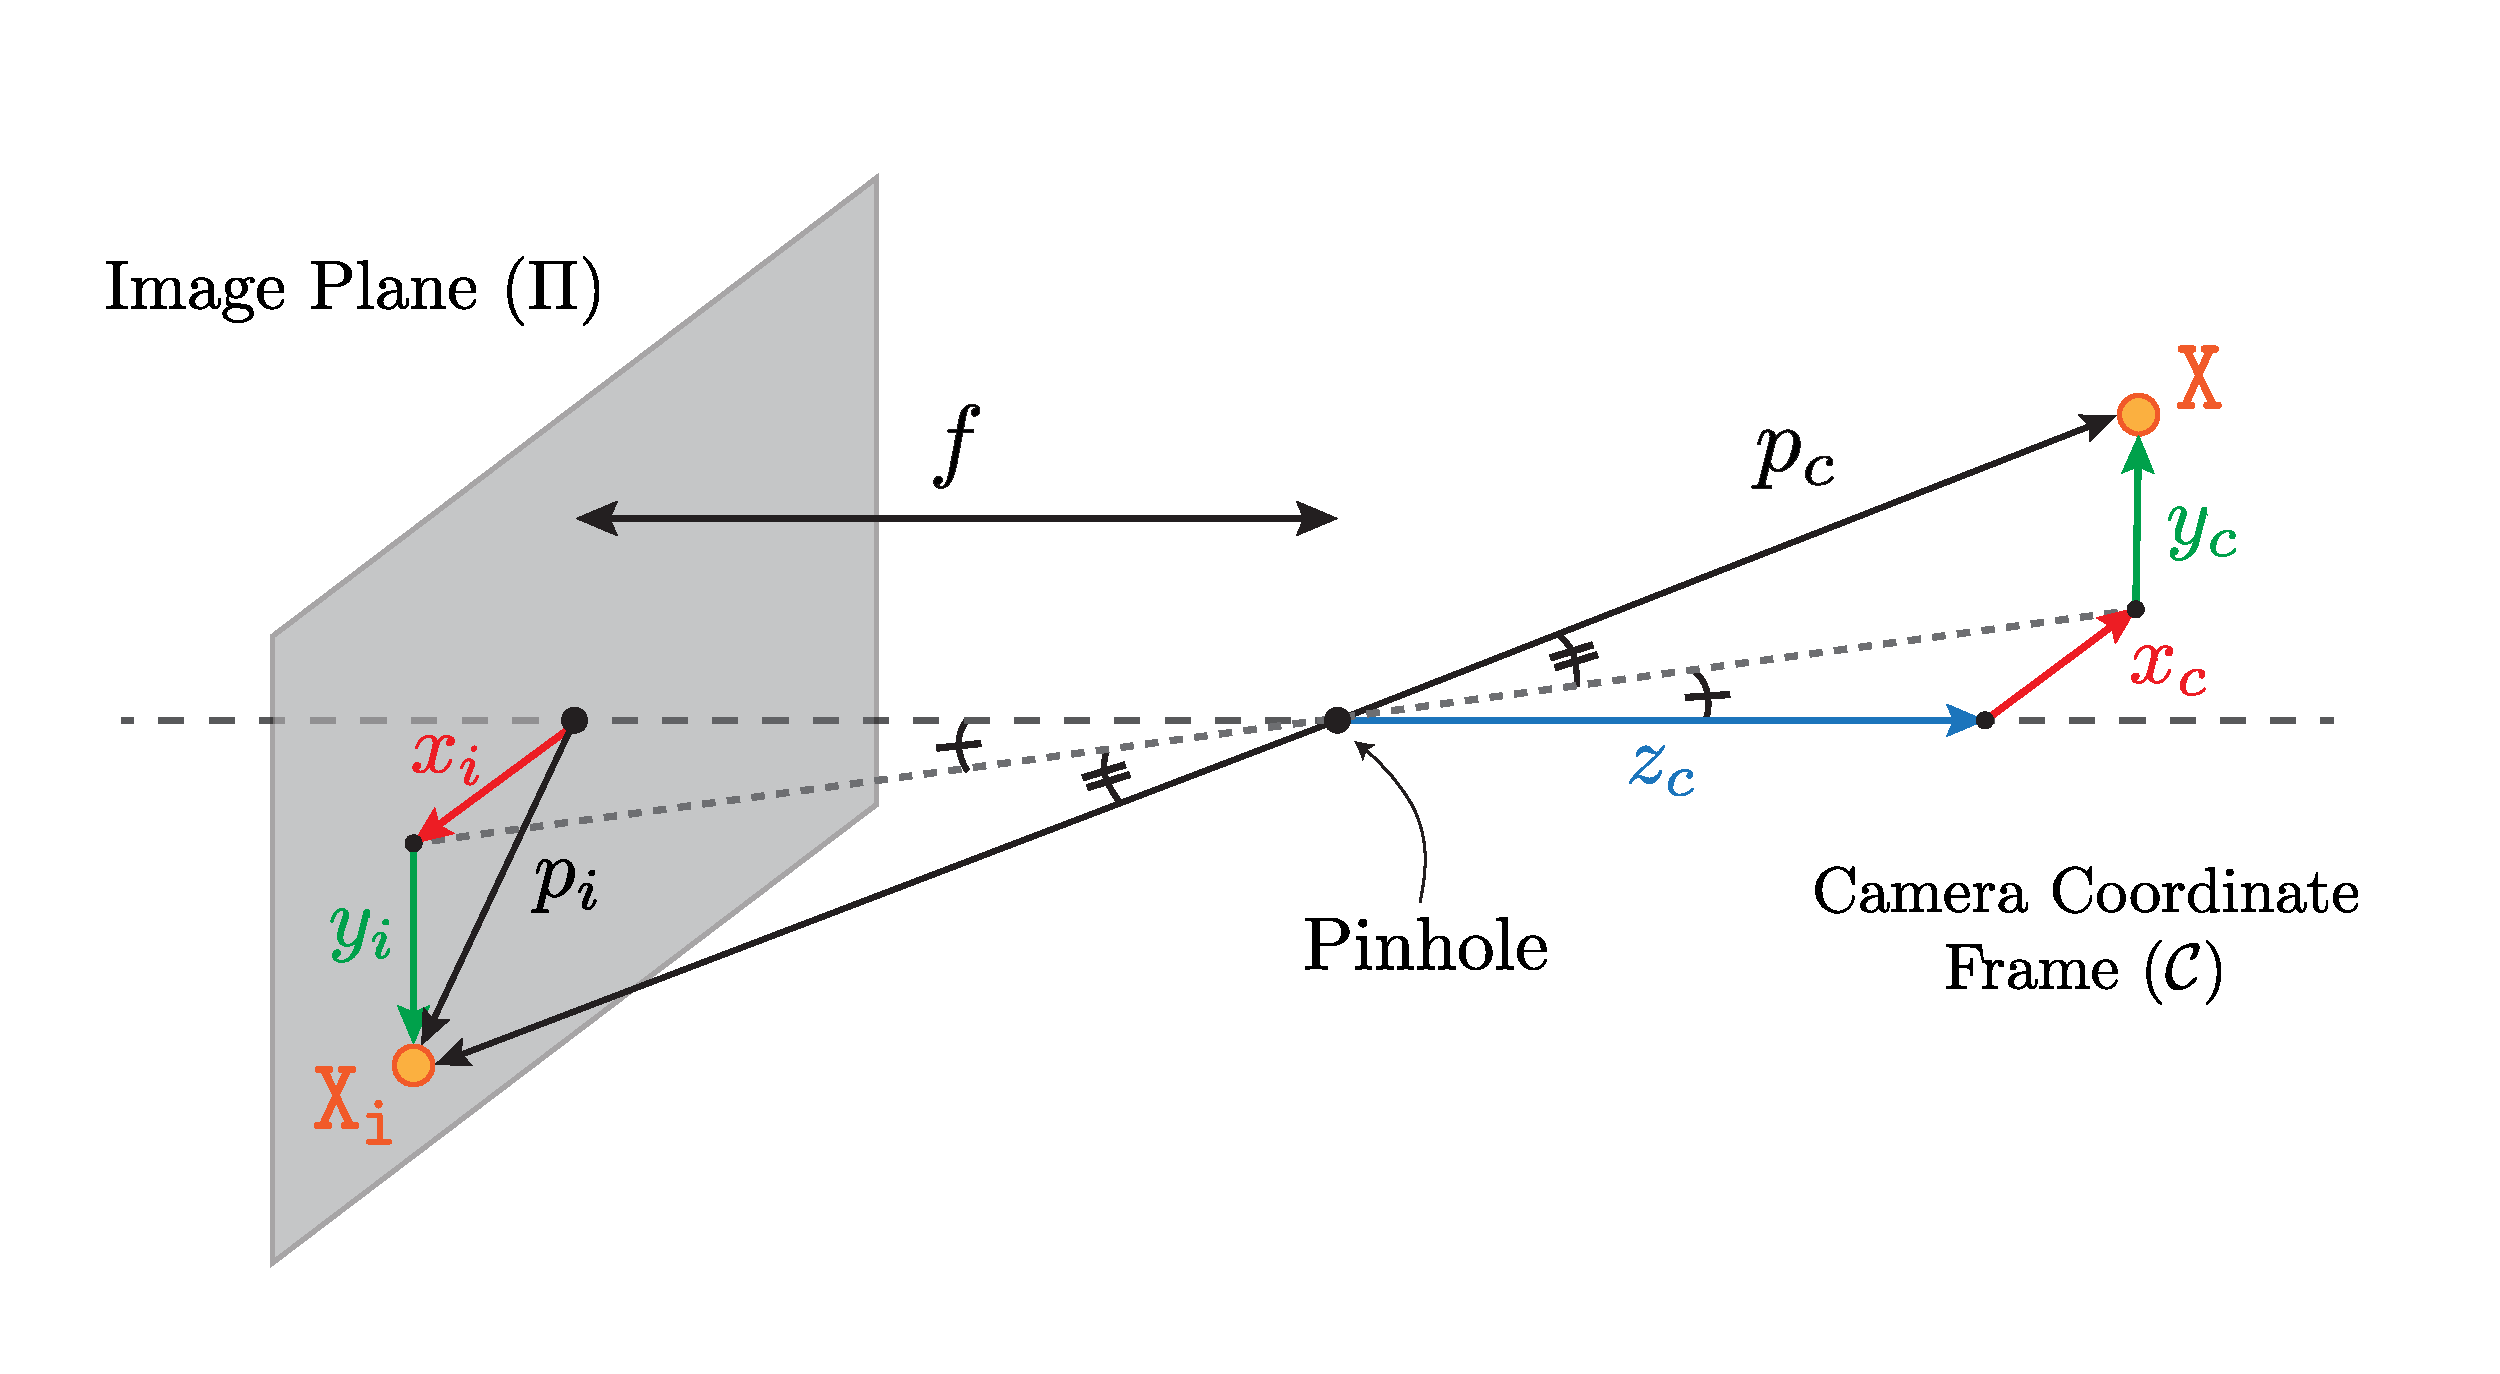
\includegraphics[width=0.9\textwidth]{diagrams/perspective_projection}
    \caption{Perspective projection of the point $\mathtt{X}$ onto the image plane $\Pi$.}
\end{figure}
When a straight line is drawn from $\mathtt{X}$ to its projection $\mathtt{X_i}$ through the aperture, it intersects the optical axis. Deconstructing this intersection in the $x$ and $y$ direction, pairs of similar triangles are formed, which relates $x_i$ to $x_c$ and $y_i$ to $y_c$.
\begin{figure}[H]
    \centering
    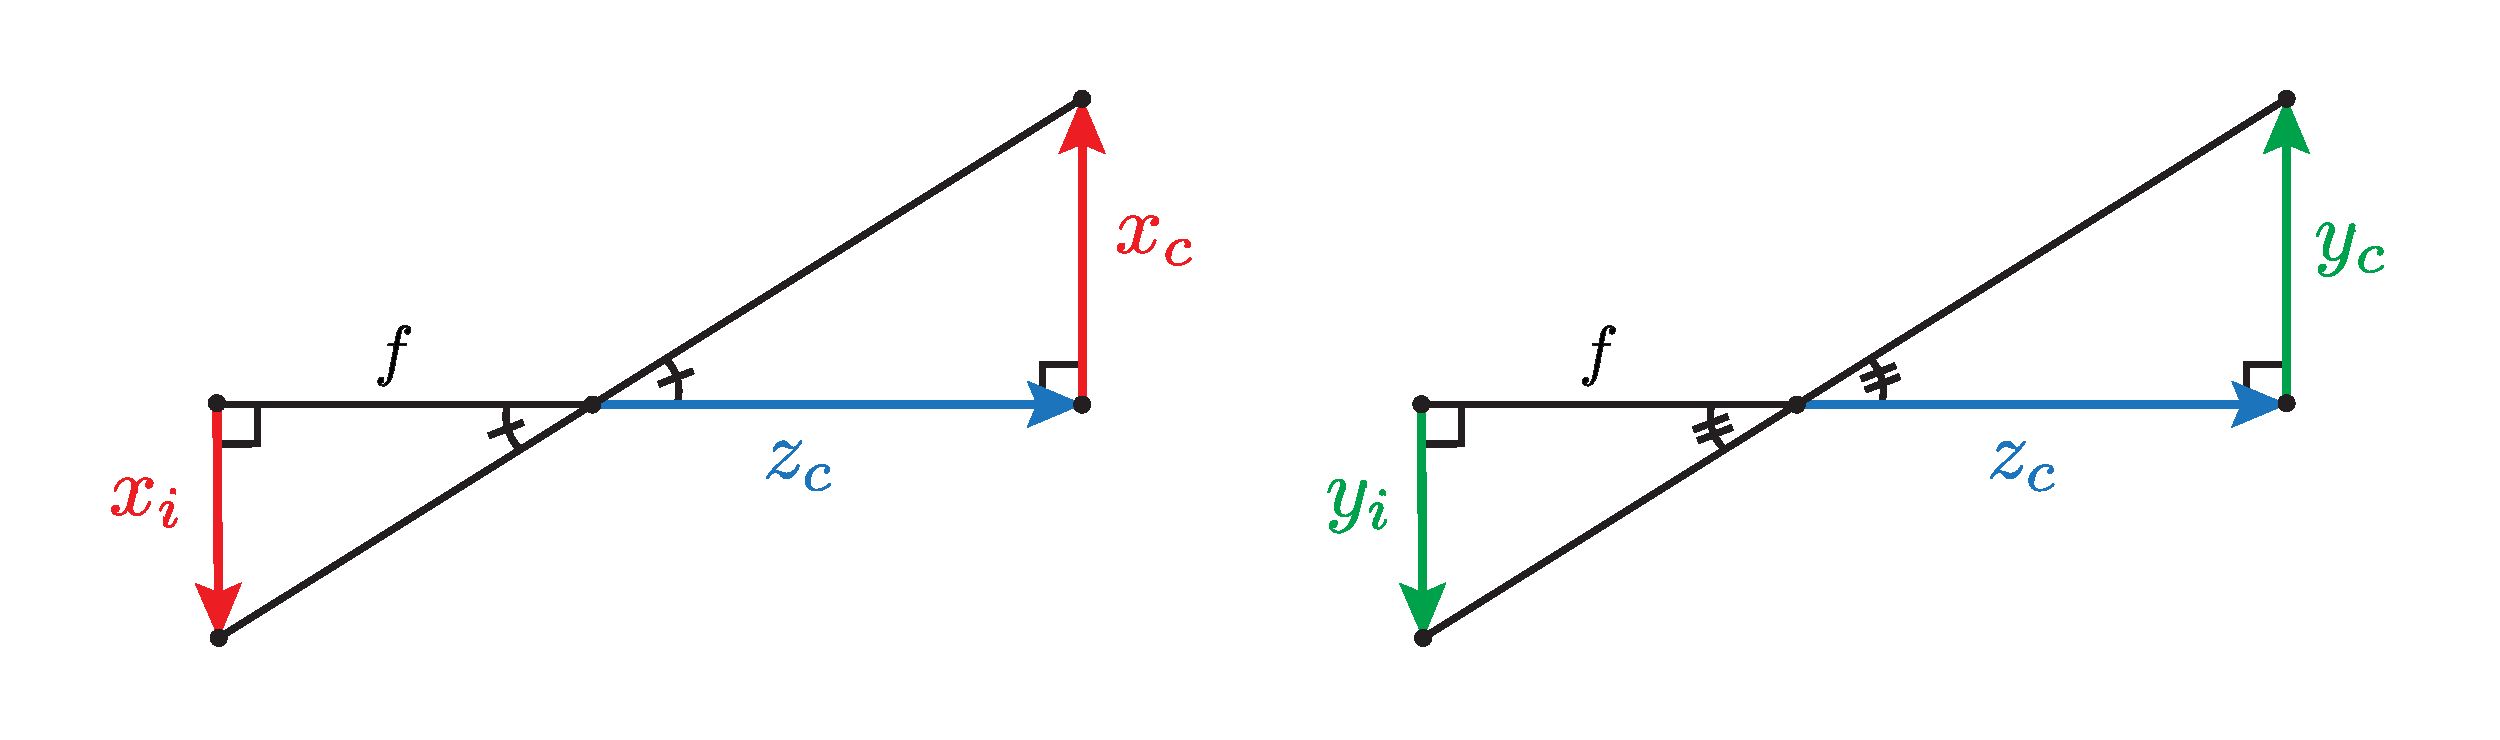
\includegraphics[width=\textwidth]{diagrams/similar_triangles}
    \caption{Similar triangles formed by perspective projection, which relate $x_i$ to $x_c$ and $y_i$ to $y_c$.} \label{fig:similar_triangles}
\end{figure}
\begin{subequations}
    \begin{gather}
        \frac{x_i}{f} = \frac{x_c}{z_c} \quad \Longrightarrow \quad x_i = f \frac{x_c}{z_c} \label{subeq:xi_result}\\
        \frac{y_i}{f} = \frac{y_c}{z_c} \quad \Longrightarrow \quad y_i = f \frac{y_c}{z_c} \label{subeq:yi_result}
    \end{gather}
\end{subequations}
Once the coordinates of the point projection, $(x_i, y_i)$, is known, we then need to convert it to actual pixel position of the point on the image, $(u, v)$. Pixel coordinates are measured in pixels, from the left-hand corner of the image. This is the convention that is typically followed in computer graphics. As such, there will be an offset in pixels, $(c_x, c_y)$, which represents the optical center of the image (i.e. the point at which the optical axis intersects the image plane). Additionally, the relationship between $(x_i, y_i)$ and $(u, v)$ is proportional, but they scale at different rates, as $(x_i, y_i)$ can be measured using any unit measurement, and can have negative and decimal values. On the other hand, $(u,v)$ are measured in discrete pixel value, which can be different sizes depending on the camera used. As such, we define scaling factors, $m_x$ and $m_y$, which represent the pixel density of the image sensor in the $x$ and $y$ axes of the image sensor plane respectively.
\begin{figure}[H]
    \centering
    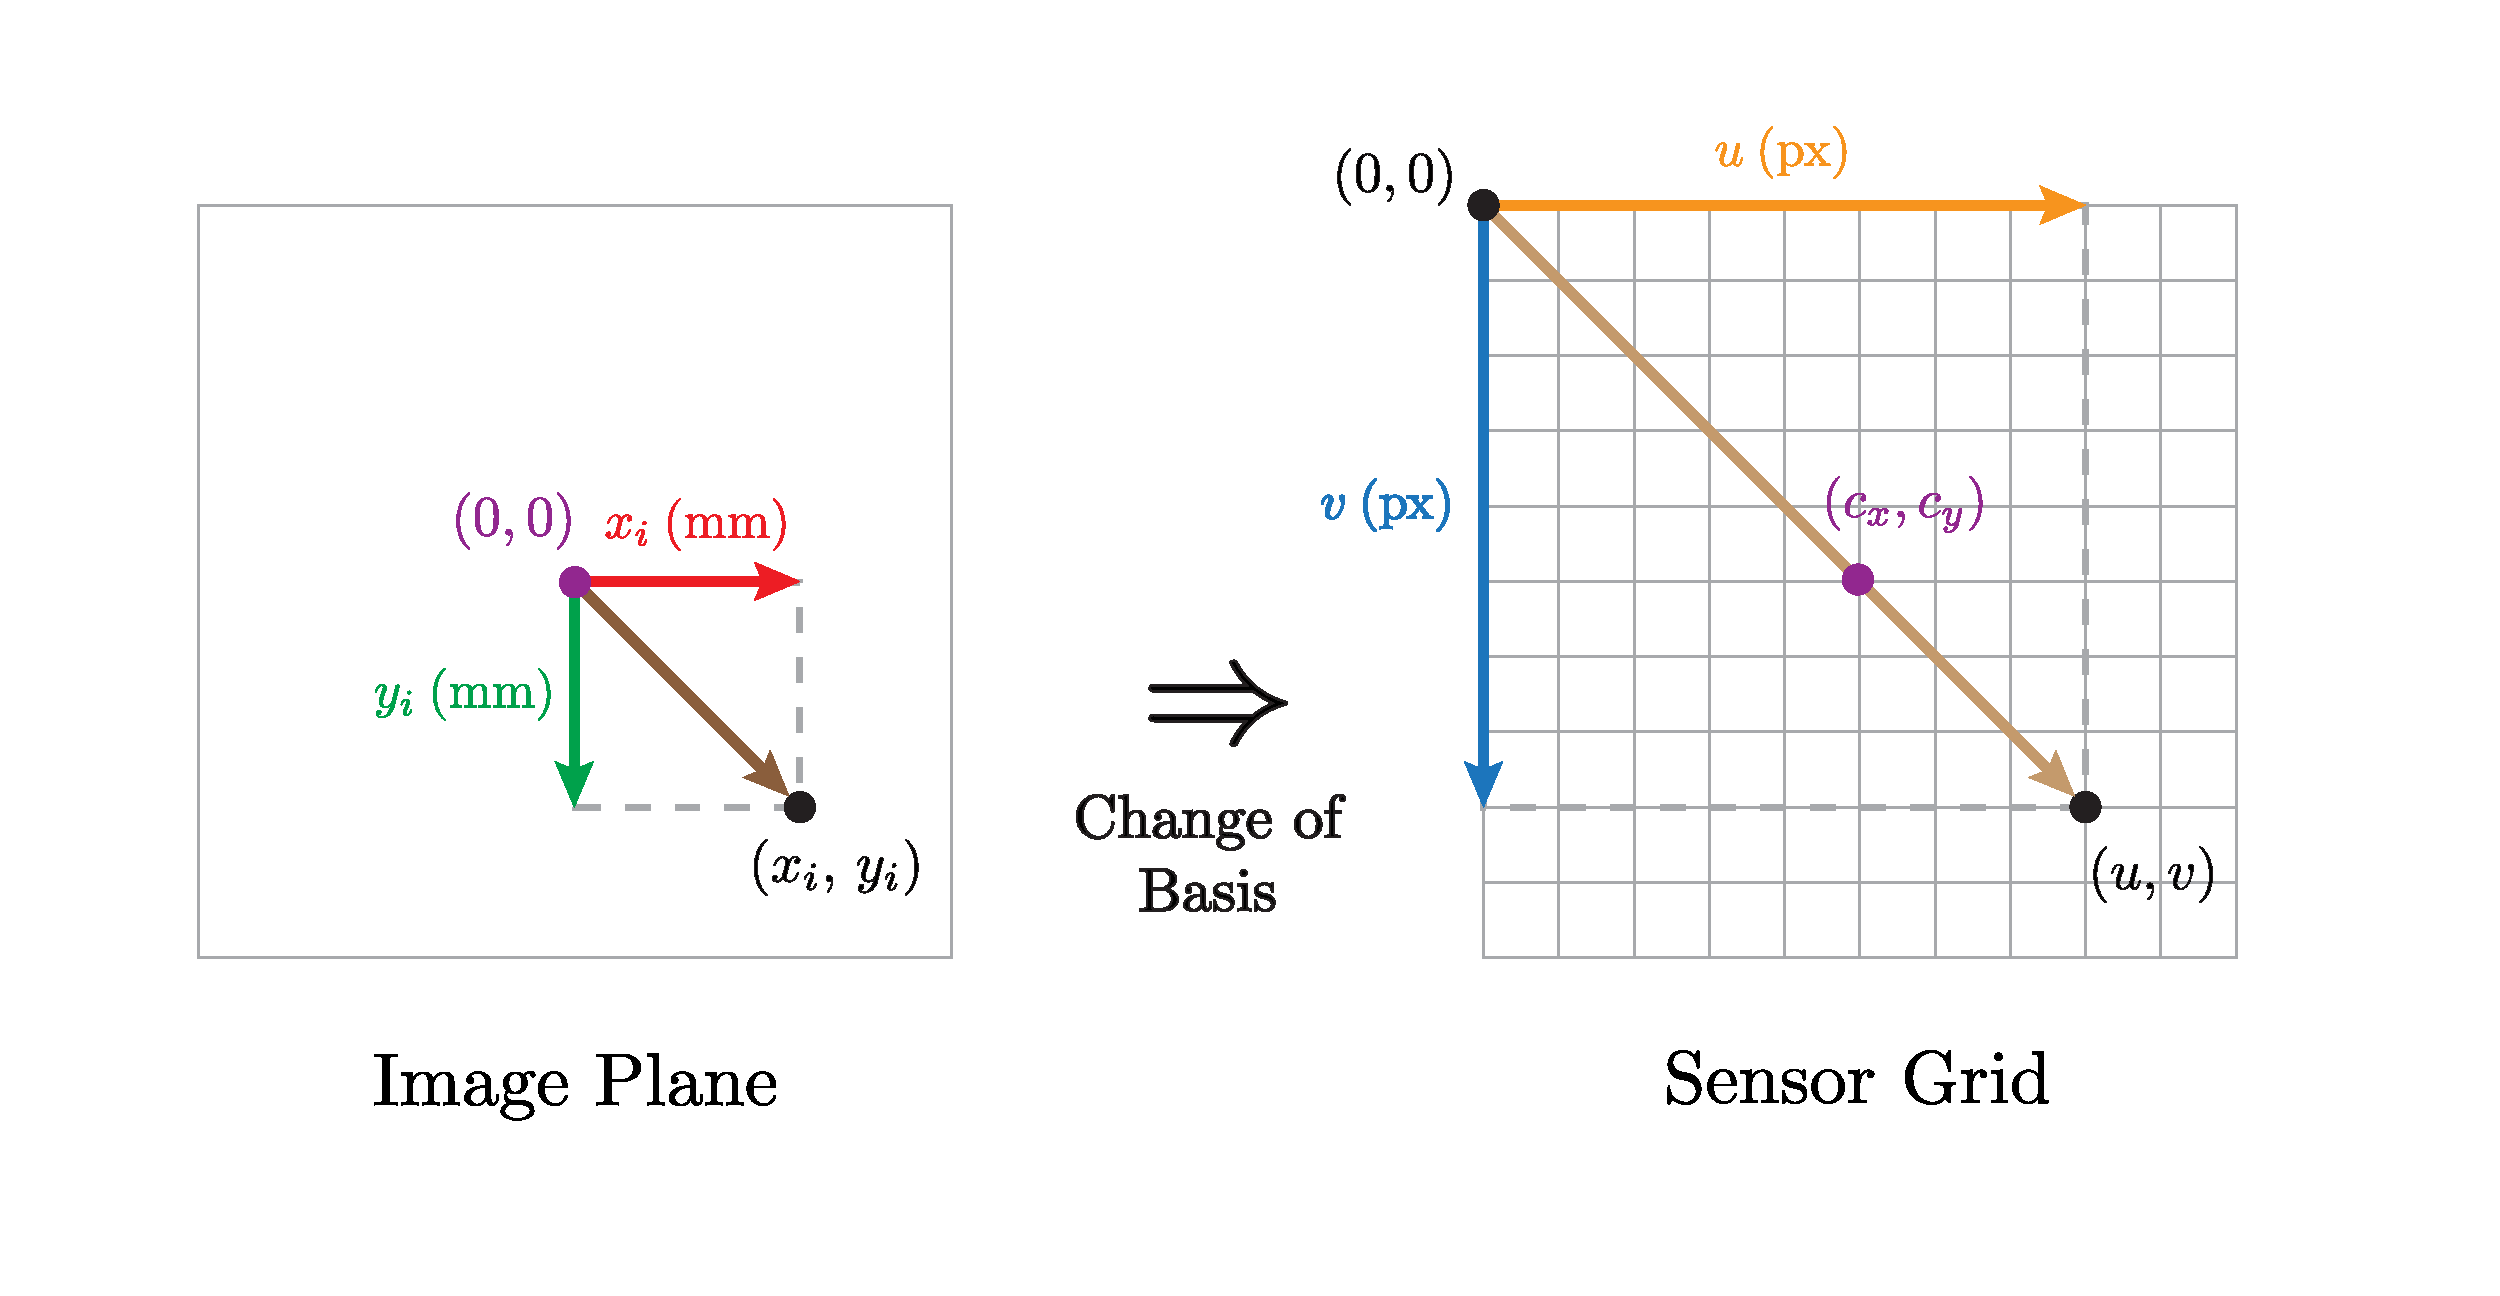
\includegraphics[width=\textwidth]{diagrams/sensor_grid}
    \caption{Conversion from image plane coordinates to sensor grid coordinates}
\end{figure}
Putting all the ideas above together, we can construct a set of linear parametric equations relating the pixel coordinates to their image coordinates thus:
\begin{align*}
    u = m_x x_i + c_x \\
    v = m_y y_i + c_y
\end{align*}
where $u, v \in \Integer^+_{\,*}$. Replacing $x_i$ and $y_i$ for the result we obtained from equations \ref{subeq:xi_result} and \ref{subeq:yi_result}, we get:
\begin{align*}
    u = m_x f \frac{x_c}{z_c} + c_x \\
    v = m_y f \frac{y_c}{z_c} + c_y
\end{align*}
This gives us a direct relationship between camera coordinates and their corresponding pixel coordinates. Since $m_x$, $m_y$, and $f$ are all unknowns, we can combine the products $m_x f$ and $m_y f$ into to $f_x$ and $f_y$ respectively. Under this new scheme, we define $f_x$ and $f_y$ as the horizontal and vertical focal lengths of camera.
\begin{gather}
    u = f_x \frac{x_c}{z_c} + c_x \\
    v = f_y \frac{y_c}{z_c} + c_y
\end{gather}
Multiply both sides of the equations by $z_c$.
\begin{subequations}
    \begin{gather*}
        z_c u = f_x x_c + z_c c_x \\
        z_c v = f_y y_c + z_c c_y
    \end{gather*}
\end{subequations}
Doing so allows us to express the relationship as a matrix transformation using \textbf{homogenous coordinates}\footnote{See Appendix \ref{sec:homogenous}.}, by letting $\widetilde{w} = z_c$.
\begin{equation}
    \begin{bmatrix}
        z_c u \\ z_c v \\ z_c
    \end{bmatrix}
    =
    a
    \begin{bmatrix}
        f_x x_c + z_c c_x \\ f_y y_c + z_c c_y \\ z_c
    \end{bmatrix}
    =
    a
    \underbrace{
        \begin{bmatrix}
            f_x & 0   & c_x \\
            0   & f_y & c_y \\
            0   & 0   & 1
        \end{bmatrix}
    }_{\mathlarger{K}}
    \begin{bmatrix}
        x_c \\ y_c \\ z_c
    \end{bmatrix}
    \eqrestriction{a \in \Real, a \neq 0}
\end{equation}
This can be represented simply with:
\begin{gather}
    \widetilde{p}_i = aK\, p_c \label{eq:pi} \eqrestriction{a \in \Real, a \neq 0}
\end{gather}
In this case, $K$ is what is known as the \textbf{calibration matrix}. It is a matrix transformation which maps a point represented in the camera coordinate frame to the coordinates of their projection onto the sensor plane.

\subsection{Extrinsic Parameters} \label{sec:extrinsics}

Extrinsic parameters describe the orientation of the camera. As such, they describe the relationship between the position of a point in the world coordinate frame and its coordinates in camera coordinates.

There are two possible types of movement affecting the orientation of the camera: rotation and translation. The rotation of the camera can be described using a $3 \times 3$ square matrix:
\begin{equation}
    R =
    \begin{bmatrix}
        r_{11} & r_{12} & r_{13} \\
        r_{21} & r_{22} & r_{23} \\
        r_{31} & r_{32} & r_{33}
    \end{bmatrix}
\end{equation}
\noindent where:
\begin{itemize}
    \item Row 1: Unit vector representing $\hat{x}_c$ after rotation.
    \item Row 2: Unit vector representing $\hat{y}_c$ after rotation.
    \item Row 3: Unit vector representing $\hat{z}_c$ after rotation.
\end{itemize}
$R$ is an orthonormal matrix, because the row and column vectors of $R$ have to be orthogonal. Orthonormality is important because it ensures that the scale of vectors do not change (meaning that determinant of $R$ has to be 1) and that the orthogonality between vectors are maintained.

\begin{figure}[H]
    \centering
    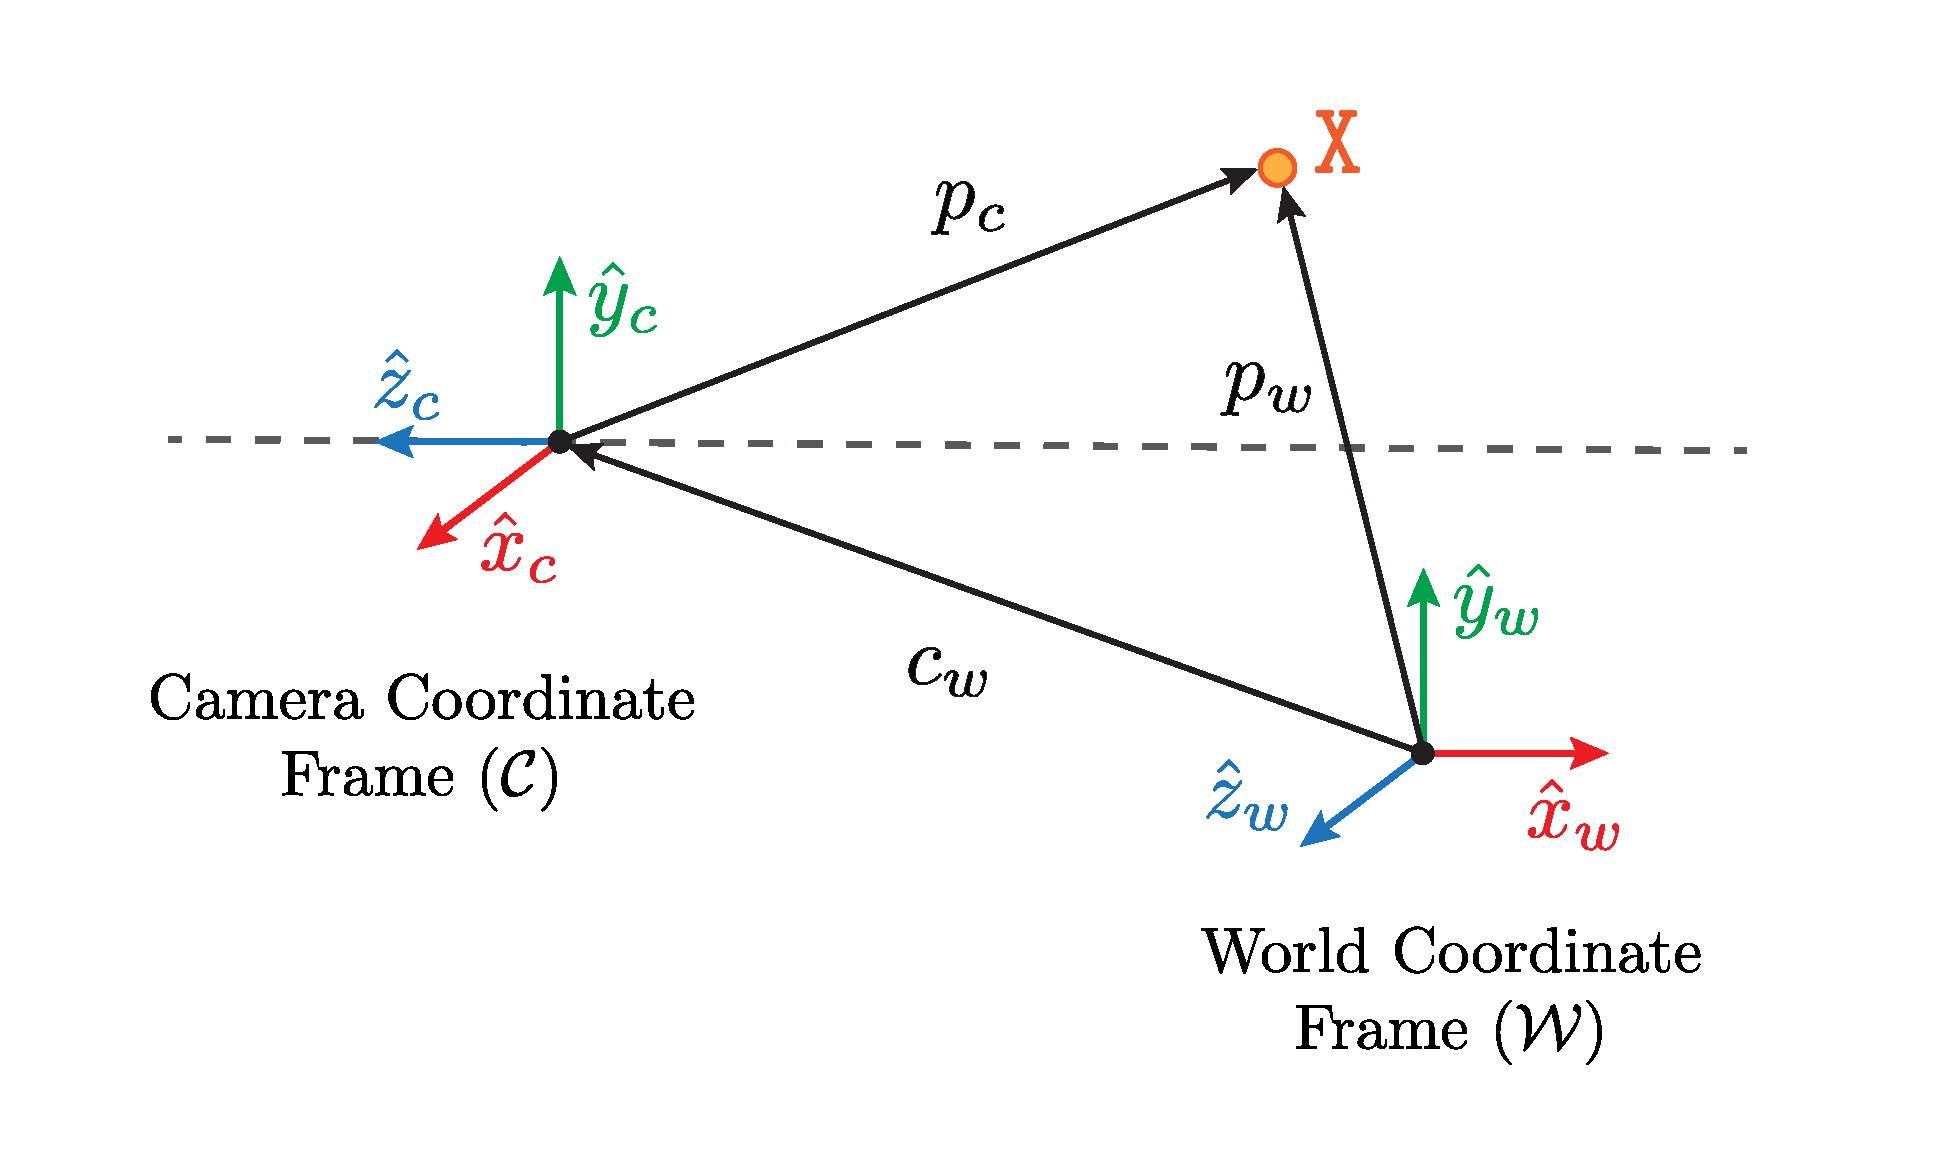
\includegraphics[width=0.9\textwidth]{diagrams/coord_transform}
    \caption{Coordinate transformation of $\mathtt{X}$ from the world coordinate frame to the camera coordinate frame.}
    \label{fig:ext}
\end{figure}

From Figure \ref{fig:ext}, we can see that the naive approach to finding the position vector of the point in $\mathcal{C}$  is equal to the position vector of the point in $\mathcal{W}$ minus the position vector of the camera $c_w$. However, the camera can be facing in other directions, and we account for this rotation by including a rotational matrix in the equation. Thus:
\begin{align}
    p_c & = R\,(p_w-c_w) \nonumber \\
        & = R\,p_w -R\,c_w
\end{align}
Since the position of the camera $c_w$ is constant, we let $t = -R\,c_w$, and $t$ represents the translation of the camera from the origin.
\begin{equation}
    p_c = R\,p_w + t
\end{equation}
This can be equivalently written as thus:
\begin{equation*}
    \begin{bmatrix}
        x_c \\ y_c \\ z_c
    \end{bmatrix}
    =
    \begin{bmatrix}
        r_{11} & r_{12} & r_{13} \\
        r_{21} & r_{22} & r_{23} \\
        r_{31} & r_{32} & r_{33}
    \end{bmatrix}
    \begin{bmatrix}
        x_w \\ y_w \\ z_w
    \end{bmatrix}
    +
    \begin{bmatrix}
        t_x \\ t_y \\ t_z
    \end{bmatrix}
\end{equation*}
We can then combine $R$ and $t$ into an augmented matrix, $[R\,|\,t\,]$, by expressing $p_w$ in homogenous coordinates.
\begin{equation}
    \begin{bmatrix}
        x_c \\ y_c \\ z_c
    \end{bmatrix}
    =
    \underbrace{
        \begin{bmatrix}
            r_{11} & r_{12} & r_{13} & t_x \\
            r_{21} & r_{22} & r_{23} & t_y \\
            r_{31} & r_{32} & r_{33} & t_z \\
        \end{bmatrix}
    }_{\mathlarger{[R\,|\,t\,]}}
    \begin{bmatrix}
        x_w \\ y_w \\ z_w \\ 1
    \end{bmatrix}
\end{equation}
Thus, we arrive at the final equation:
\begin{equation}
    p_c=[R\,|\,t\,] \,\widetilde{p}_w \label{eq:pc}
\end{equation}


\section{Projection Matrix} \label{sec:projection}

When we combine the equation for the intrinsic transformation, $\widetilde{p}_i = aK\,p_c$ for $a \in \Real$ and $a \neq 0$ (eq. \ref{eq:pi}), with the equation for the extrinsic transformation, $p_c = [R\,|\,t\,]\,\widetilde{p}_w$ (eq. \ref{eq:pc}), we obtain:
\begin{equation} \label{eq:combined}
    \widetilde{p}_{i} = aK\,[R\,|\,t\,]\,\widetilde{p}_{w} \eqrestriction{a \in \Real, a \neq 0}
\end{equation}

This single equation encapsulates the relationship between the world coordinates and its corresponding pixel coordinates. We can then further simplify our camera model by defining a new matrix, $P$, which is equivalent to the product $K\,[R\,|\,t\,]$. Since $K$ is a $3 \times 3$ matrix and $[R\,|\,t\,]$ is a $3 \times 4$ matrix, the matrix product $K[R\,|\,t\,]$ yields a $3 \times 4$ matrix. 
\begin{equation}
    \underbrace{
        \begin{bmatrix}
        p_{11} & p_{12} & p_{13} & p_{14} \\
        p_{21} & p_{22} & p_{23} & p_{24} \\
        p_{31} & p_{32} & p_{33} & p_{34}
    \end{bmatrix}
    }_{\mathlarger{P}}
    \equiv
    a
    \underbrace{
        \begin{bmatrix}
            f_x & 0   & c_x \\
            0   & f_y & c_y \\
            0   & 0   & 1
        \end{bmatrix}
    }_{\mathlarger{K}}
    \underbrace{
        \begin{bmatrix}
            r_{11} & r_{12} & r_{13} & t_x \\
            r_{21} & r_{22} & r_{23} & t_y \\
            r_{31} & r_{32} & r_{33} & t_z \\
        \end{bmatrix}
    }_{\mathlarger{[R\,|\,t\,]}}
\end{equation}
Replacing $P$ for $K\,[R\,|\,t\,]$ in equation \ref{eq:combined}, we obtain:
\begin{equation} \label{eq:project}
    \widetilde{p}_{i} = aP\,\widetilde{p}_{w}
\end{equation}
Equivalently:
\begin{equation} \label{eq:proj}
    \begin{bmatrix}
        \widetilde{u}_n \\ \widetilde{v}_n \\ \widetilde{w}_n
    \end{bmatrix}
    =
    a
    \begin{bmatrix}
        p_{11} & p_{12} & p_{13} & p_{14} \\
        p_{21} & p_{22} & p_{23} & p_{24} \\
        p_{31} & p_{32} & p_{33} & p_{34}
    \end{bmatrix}
    \begin{bmatrix}
        x_w^{(n)} \\ y_w^{(n)} \\ z_w^{(n)} \\ 1
    \end{bmatrix}
\end{equation}
where $n \in \Natural$ denotes the n\textsuperscript{th} point.

The implications of this equation is very important, as it means that a $3 \times 4$ matrix is sufficient in describing the relationship between a point in the world coordinate frame to its projection onto the image plane in pixel coordinates.

\subsection{Solving for the Projection Matrix}

Now, we need to devise a way to solve for the projection matrix. Since we know that the projection matrix describes relationship between a point and their projection, we can go backwards and solve for the projection matrix given a set of points and their corresponding image projections. Rewriting the matrix equation \ref{eq:project} as a set of parametric equations and letting $a=1$ for now, we obtain:
\begin{align*}
    \widetilde{u}_n = p_{11}x_w^{(n)} + p_{12}y_w^{(n)} + p_{13}z_w^{(n)} + p_{14} \\
    \widetilde{v}_n = p_{21}x_w^{(n)} + p_{22}y_w^{(n)} + p_{23}z_w^{(n)} + p_{24} \\
    \widetilde{w}_n = p_{31}x_w^{(n)} + p_{32}y_w^{(n)} + p_{33}z_w^{(n)} + p_{34}
\end{align*}
We convert the set of equations back to their inhomogeneous form by recognizing the fact that $u_n = \nicefrac{\widetilde{u}_n}{\widetilde{w}_n}$ and $v_n = \nicefrac{\widetilde{v}_n}{\widetilde{w}_n}$. 
\begin{align*}
    u_n & = \frac{p_{11}x_w^{(n)} + p_{12}y_w^{(n)} + p_{13}z_w^{(n)} + p_{14}}{p_{31}x_w^{(n)} + p_{32}y_w^{(n)} + p_{33}z_w^{(n)} + p_{34}} \\
    v_n & = \frac{p_{21}x_w^{(n)} + p_{22}y_w^{(n)} + p_{23}z_w^{(n)} + p_{24}}{p_{31}x_w^{(n)} + p_{32}y_w^{(n)} + p_{33}z_w^{(n)} + p_{34}}
\end{align*}
For both equations, multiply both sides by the denominator.
\begin{align*}
    u_n(p_{31}x_w^{(n)} + p_{32}y_w^{(n)} + p_{33}z_w^{(n)} + p_{34}) = p_{11}x_w^{(n)} + p_{12}y_w^{(n)} + p_{13}z_w^{(n)} + p_{14} \\
    v_n(p_{31}x_w^{(n)} + p_{32}y_w^{ (n)} + p_{33}z_w^{(n)} + p_{34}) = p_{21}x_w^{(n)} + p_{22}y_w^{(n)} + p_{23}z_w^{(n)} + p_{24}
\end{align*}
Bringing all the terms onto one side:
\begin{subequations}
    \begin{align}
        0 = p_{11}x_w^{(n)} + p_{12}y_w^{(n)} + p_{13}z_w^{(n)} + p_{14} - p_{31}u_nx_w^{(n)} - p_{32}u_ny_w^{(n)} - p_{33}u_nz_w^{(n)} - p_{34}u_n \\
        0 = p_{21}x_w^{(n)} + p_{22}y_w^{(n)} + p_{23}z_w^{(n)} + p_{24} - p_{31}v_nx_w^{(n)} - p_{32}v_ny_w^{(n)} - p_{33}v_nz_w^{(n)} - p_{34}v_n
    \end{align}
\end{subequations}
$p$ has 12 degrees of freedom, and since each point generates a distinct set of the two equations above, a minimum of 6 sets of points and their corresponding image projections are necessary in order to solve the system. These equations form a system of equations, which can be rewritten in the form of a matrix equation:
\setcounter{MaxMatrixCols}{20}
\begin{equation}
    \scalemath{0.9}{
    \begin{bmatrix}
        0 \\ 0 \\ 0 \\ 0 \\ 0 \\ 0 \\ 0 \\ 0 \\ 0 \\ 0 \\ 0 \\ 0
    \end{bmatrix}
    =
    \underbrace{
        \begin{blockarray}{[*{12}c]}
            x_w^{(1)} & y_w^{(1)} & z_w^{(1)} & 1 & 0         & 0         & 0         & 0 & -u_1 x_w^{(1)} & -u_1 y_w^{(1)} & -u_1 z_w^{(1)} & -u_1 \\
            0         & 0         & 0         & 0 & x_w^{(1)} & y_w^{(1)} & z_w^{(1)} & 1 & -v_1 x_w^{(1)} & -v_1 y_w^{(1)} & -v_1 z_w^{(1)} & -v_1 \\
            \BAmulticolumn{6}{c}{\vdots} & \BAmulticolumn{6}{c}{\vdots} \\
            x_w^{(n)} & y_w^{(n)} & z_w^{(n)} & 1 & 0         & 0         & 0         & 0 & -u_n x_w^{(n)} & -u_n y_w^{(n)} & -u_n z_w^{(n)} & -u_n \\
            0         & 0         & 0         & 0 & x_w^{(n)} & y_w^{(n)} & z_w^{(n)} & 1 & -v_n x_w^{(n)} & -v_n y_w^{(n)} & -v_n z_w^{(n)} & -v_n
        \end{blockarray}
    }_{\mathlarger{G}}
    \underbrace{
        \begin{bmatrix}
            p_{11} \\ p_{12} \\ p_{13} \\ p_{14} \\ p_{21} \\ p_{22} \\ p_{23} \\ p_{24} \\ p_{31} \\ p_{32} \\ p_{33} \\ p_{34}
        \end{bmatrix}
    }_{\mathlarger{p}}
    }
\end{equation}
where $G$ is a $2n \times 12$ matrix, $n \in \Integer^+$, and $p$ is the matrix vectorization of $P$. When using 6 correspondences, a unique solution can be obtained using classical approaches, such as using 
\textbf{Gaussian elimination}. But since we want to minimize uncertainty and achieve a solution which is as accurate as possible, we want to use as many correspondences as possible. When using more the 6 correspondences, we have more equations than unknowns. Such systems are \emph{overdetermined}, and generally have no solutions \footcite{williamsOverdeterminedSystems1990}. However, we can optimize the system and obtain the ``best approximate solution'' using a method such as the \hyperref[sec:clss]{\textbf{least-squares method}}. 

\subsection{Constrained Least-Squares Solution} \label{sec:clss}

First, we must clarify what a ``best approximate solution'' is. 
\begin{definition}
    Let $A$ be an $m \times n$ matrix and let $b$ be a vector in $\Real^m$. A \textbf{least-squares solution} of the matrix equation $Ax = b$ is a vector $\widehat{x}$ such that:
    \begin{equation*}
        \mathrm{dist}(b, A\widehat{x}) \leq \mathrm{dist}(b, Ax) \qquad \forall x \in \Real^m
    \end{equation*}
\end{definition}

The term least-squares solution comes from the fact that $\mathrm{dist}(b, A\widehat{x})= \Vert b - A\widehat{x} \Vert$ is the square root of the sum of the squares of the entries of the vector $b - A\widehat{x}$. In other words, a least-squares solution solve a matrix equation as closely as possible by minimizing the sum of the squares of the differences between the entries of $A\widehat{x}$ and $b$. \footcite{margalitMethodLeast}

Returning to our specific problem, we can apply least-squares method by minimizing $\Vert Gp \Vert^2$. We minimize $\Vert Gp \Vert^2$ because we recognize that minimizing the square of the magnitude is equivalent to minimizing the magnitude itself, and that for a given vector $v$, it is easier to compute $\Vert v \Vert^2$ instead of $\Vert v \Vert$ since it eliminates the square root:
\begin{equation*}
    \Vert v \Vert^2
     = \left(\sqrt{v_1^2+v_2^2+ \cdots v_n^2}\right)^2 
     = v_1^2+v_2^2+ \cdots v_n^2 
     = \begin{bmatrix}
        v_1 & v_2 & \cdots & v_n
    \end{bmatrix}
    \begin{bmatrix}
        v_1 \\ v_2 \\ \vdots \\ v_n
    \end{bmatrix} 
     = v^\T v
\end{equation*}
$v^\T$ represents the \emph{transpose} of $v$, i.e. swapping its rows and columns, transforming a row vector into a column vector or vice versa.

However, we need to further constrain the problem since the projection matrix $P$ is applied onto homogeneous coordinates, where the property holds that multiplying the homogeneous coordinate of a point by a non-zero scalar still represents the same point\footnote{See Appendix \ref{sec:homogeneous}.}. This means that there is an infinite amount of solutions, because once we have found a valid solution for $P$, we can always multiply $P$ by a non-zero scalar $k$ and still yield a valid solution, i.e. $P \equiv kP$. As such, any solution for $P$ is only defined to a certain scale factor $k$. To mitigate this, we arbitrarily set the condition that $\Vert p \Vert^2$ must equal 1. Thus:
\begin{equation*} \label{eq:min1}
    \optmin{p}{\lVert Gp \rVert^2}{\lVert p \rVert^2 = 1}
\end{equation*}
Or equivalently:
\begin{equation} \label{eq:min2}
    \optmin{p}{\left(p^\T G^\T Gp\right)}{p^\T p = 1}
\end{equation}
The \emph{Lagrangian} \footcite[][2]{ghojoghEigenvalueGeneralized2023} of this equation is:
\begin{equation}
    \mathcal{L}(p, \lambda) = p^\T G^\T Gp - \lambda \left( p^\T p - 1 \right)
\end{equation}
where $\lambda \in \mathbb{R}$ is the \emph{Lagrange multiplier}. Since $p$ is minimized when $\mathcal{L}$ is minimized, we want to find the absolute minimum of $\mathcal{L}$. As such, we need to locate the critical points of $\mathcal{L}$. To find these points, we want to look for values of $p$ and $\lambda$ where all partial derivatives (denoted using $\partial$) of the Lagrangian are zero.
\begin{gather}
    \frac{\partial}{\partial p}\mathcal{L}(p, \lambda) \seteq 0 \nonumber\\
    \Rightarrow \frac{\partial}{\partial p} \left[ p^\T G^\T Gp - \lambda \left( p^\T p - 1 \right) \right] = 0 \nonumber \\
    \Rightarrow 2G^\T Gp - 2 \lambda p = 0 \nonumber \\
    \Rightarrow G^\T Gp = \lambda p \label{eq:eigen}
\end{gather}
This equation is in fact in the form of the eigenvalue problem for $G^\T G$. Potential solutions for $p$ are eigenvectors that satisfy equation \ref{eq:eigen}, with the scalar $\lambda \in \mathbb{R}$ as the eigenvalue. Since this is a minimization problem, the best approximate solution to $p$ is the one which has the smallest $\lambda$. \footcite[][2]{ghojoghEigenvalueGeneralized2023}

\section{Extracting Parameters} \label{sec:extract}

Once we have solved for the projection for the projection matrix $P$, we can then decompose it and extract the intrinsic and extrinsic parameters. 

\begin{align}
    P & = K\,[\,R\;|\;t\,]       \nonumber \\
      & = K\,[\,R\;|\;-Rc_w\,]   \nonumber \\
      & = [\,KR\;|\;-KRc_w\,]              \\
\end{align}



\subsection{RQ Decomposition} \label{subsec:rq}

\begin{equation*}
    Q =
    \begin{bmatrix}
        p_{11} & p_{12} & p_{13} \\
        p_{21} & p_{22} & p_{23} \\
        p_{31} & p_{32} & p_{33}
    \end{bmatrix}
    =
    \underbrace{
        \begin{bmatrix}
            f_x & 0   & c_x \\
            0   & f_y & c_y \\
            0   & 0   & 1
        \end{bmatrix}
    }_{\mathlarger{K}}
    \underbrace{
        \begin{bmatrix}
            r_{11} & r_{12} & r_{13} \\
            r_{21} & r_{22} & r_{23} \\
            r_{31} & r_{32} & r_{33} \\
        \end{bmatrix}
    }_{\mathlarger{R}}
\end{equation*}

Since $K$ is in the form of an \emph{upper right triangular matrix} and $R$ is an \emph{orthonormal matrix}, we can find unique solutions for $K$ and $R$ using a method called \emph{RQ decomposition}.



\emph{RQ decomposition} is a technique which allows us to uniquely decompose a matrix $A$ into a product $A=RQ$, where $R$ is an upper

Since

\subsection{Extracting the Translation Vector}

\begin{gather}
    -Qc_w =
    \begin{bmatrix}
        p_{14} \\ p_{24} \\ p_{34}
    \end{bmatrix} \nonumber \\
    \Rightarrow c_w = -Q^{-1}
    \begin{bmatrix}
        p_{14} \\ p_{24} \\ p_{34}
    \end{bmatrix}
\end{gather}




\subsection{Extracting Orientation as Angles}

When constructing the extrinsic matrix in section \ref{sec:extrinsics}, we defined the rotation of the camera as a $3 \times 3$ matrix, where the

We can represent the rotation in terms of \emph{Tait-Bryan Angles}, where the rotation is represented as 3 elemental rotations about each of the principle axes.

\begin{subequations}
    \begin{gather}
        R_x(\alpha) =
        \begin{bmatrix}
            1 & 0            & 0             \\
            0 & \cos(\alpha) & -\sin(\alpha) \\
            0 & \sin(\alpha) & \cos(\alpha)
        \end{bmatrix} \\
        R_y(\beta) =
        \begin{bmatrix}
            \cos(\beta)  & 0 & -\sin(\beta) \\
            0            & 1 & 0            \\
            -\sin(\beta) & 0 & -\cos(\beta)
        \end{bmatrix} \\
        R_z(\gamma) =
        \begin{bmatrix}
            \cos(\gamma) & -\sin(\gamma) & 0 \\
            \sin(\gamma) & \cos(\gamma)  & 0 \\
            0            & 0             & 1
        \end{bmatrix}
    \end{gather}
\end{subequations}


\begin{equation}
    R \equiv R_z(\gamma)R_y(\beta)R_x(\alpha)
\end{equation}

\begin{align}
    R & =
    \begin{bmatrix}
        0 & \cos(\alpha) & -\sin(\alpha) \\
        0 & \sin(\alpha) & \cos(\alpha)  \\
        1 & 0            & 0             \\
    \end{bmatrix}
    \begin{bmatrix}
        \cos(\beta)  & 0 & -\sin(\beta) \\
        0            & 1 & 0            \\
        -\sin(\beta) & 0 & -\cos(\beta)
    \end{bmatrix}
    \begin{bmatrix}
        \cos(\gamma) & -\sin(\gamma) & 0 \\
        \sin(\gamma) & \cos(\gamma)  & 0 \\
        0            & 0             & 1
    \end{bmatrix} \nonumber \\
      & =
    \scalemath{0.85}{
        \begin{bmatrix}
            \cos(\beta)\,\cos(\gamma) & \sin(\alpha)\,\sin(\beta)\,\cos(\gamma) - \cos(\alpha)\,\sin(\gamma) & \cos(\alpha)\,\sin(\beta)\,\cos(\gamma) + \sin(\alpha)\,\cos(\gamma) \\
            \cos(\beta)\,\sin(\gamma) & \sin(\alpha)\,\sin(\beta)\,\sin(\gamma) + \cos(\alpha)\,\cos(\gamma) & \cos(\alpha)\,\sin(\beta)\,\sin(\gamma) - \sin(\alpha)\,\cos(\gamma) \\
            -\sin(\beta)              & \sin(\alpha)\,\cos(\beta)                                            & \cos(\alpha)\,\cos(\beta)
        \end{bmatrix}
    }
\end{align}

We have that
\begin{equation*}
    r_{31} = -\sin(\beta) \nonumber
\end{equation*}
\begin{equation}
    \Rightarrow \beta = \sin^{-1}(-r_{31})
\end{equation}

\begin{equation*}
    r_{32} = \sin(\alpha)\cos(\beta)
\end{equation*}
\begin{align}
    \begin{split}
        \Rightarrow \alpha & = \sin^{-1}\left(\frac{r_{32}}{\cos(\beta)}\right)               = \sin^{-1}\left(\frac{r_{32}}{\cos(\sin^{-1}(-r_{31}))}\right) \\
        & = \sin^{-1}\left(\frac{r_{32}}{\sqrt{1-r_{31}^2}}\right)
    \end{split}
\end{align}

\begin{equation*}
    r_{21} = \cos(\beta)\sin(\gamma)
\end{equation*}
\begin{align}
    \begin{split}
        \Rightarrow \gamma & = \sin^{-1}\left(\frac{r_{21}}{\cos(\beta)}\right)               = \sin^{-1}\left(\frac{r_{21}}{\cos(\sin^{-1}(-r_{31}))}\right) \\
        & = \sin^{-1}\left(\frac{r_{21}}{\sqrt{1-r_{31}^2}}\right)
    \end{split}
\end{align}



\section{Experimental Validation}

To demonstrate the effectiveness of the model, I conducted tests by applying it to calibrate three different cameras: the Canon EOS D80, the iPhone X, and the Nikon D100. These cameras were chosen because they vary widely in terms of construction, image quality, and level of distortion. This diverse set of cameras provides a robust evaluation platform, allowing for an empirical assessment of the model's calibration performance, despite the small and statistically insignificant sample size.

To calibrate the camera, I first captured a picture of the calibration object of known dimensions using each of the cameras. In this case, the calibration object used consisted of 3 orthogonal planes with a checkerboard pattern imprinted onto each of the planes. The points at which the planes intersect was chosen to be the origin point of the world scene.

\begin{figure}[H]
    \centering
    \begin{subfigure}{0.5\textwidth}
        \centering
        \includegraphics[width=0.8\textwidth]{images/cal_object.png}
    \end{subfigure}%
    \begin{subfigure}{0.5\textwidth}
        \centering
        \includegraphics[width=0.9\textwidth]{images/cal_planes.png}
    \end{subfigure}
    \caption{Custom-made calibration object made using laser-cut MDF board. The checkerboard pattern was printed onto paper and glued onto the boards.}
\end{figure}

Then, I extracted the pixel coordinates of each of the points on the checkerboard and paired them to their corresponding real-world coordinates. This forms our dataset, which was then fed into a self-developed \emph{Python} program named \texttt{calicam}\footnote{See Appendix \ref{sec:source} for the source code of \texttt{calicam}.}. A subset of the dataset was earmarked to calibrate the model, used to solve for the projection matrix and extract intrinsic and extrinsic parameters. The remaining points were utilized for validation; the program reprojects these points and compares the estimated pixel coordinates of the projections to the ground truth provided in the dataset. By taking the average distances between the predicted points and their ground truths, we essentially calculate the reprojection error of the model, providing a quantitative measure of the accuracy of the predicted image coordinates compared to the actual observed values.

\begin{table}[H]
    \centering
    \resizebox{\columnwidth}{!}{
    \begin{tabular}{p{3cm}ccccccc}
        \toprule
                                                         &             & \multicolumn{2}{c}{\textbf{\small CANON D80}} & \multicolumn{2}{c}{\textbf{\small IPHONE X}} & \multicolumn{2}{c}{\textbf{\small NIKON D100}}                                                                               \\
        \cmidrule(lr){3-4}
        \cmidrule(lr){5-6}
        \cmidrule(lr){7-8}
                                                         &             & Spreaded Out                                  & Concentrated                                 & Spreaded Out                                   & Concentrated            & Spreaded Out            & Concentrated            \\
        \midrule
        \addlinespace
        \multirow{2}{*}{\footnotesize Focal Lengths}     & $f_x$       & $\qty{8404.1}{\pixel}$                        & $\qty{8305.9}{\pixel}$                       & $\qty{3281.5}{\pixel}$                         & $\qty{3125.7}{\pixel}$  & $\qty{8144.4}{\pixel}$  & $\qty{7716.4}{\pixel}$  \\
                                                         & $f_y$       & $\qty{8387.9}{\pixel}$                        & $\qty{8338.1}{\pixel}$                       & $\qty{3279.9}{\pixel}$                         & $\qty{3137.8}{\pixel}$  & $\qty{8142.6}{\pixel}$  & $\qty{7755.5}{\pixel}$  \\
        \addlinespace
        \multirow{2}{*}{\footnotesize Principal Point}   & $c_x$       & $\qty{3151.6}{\pixel}$                        & $\qty{3400.0}{\pixel}$                       & $\qty{2043.0}{\pixel}$                         & $\qty{2031.4}{\pixel}$  & $\qty{1541.8}{\pixel}$  & $\qty{1851.5}{\pixel}$  \\
                                                         & $c_y$       & $\qty{1972.8}{\pixel}$                        & $\qty{2075.8}{\pixel}$                       & $\qty{1453.1}{\pixel}$                         & $\qty{1467.4}{\pixel}$  & $\qty{1027.9}{\pixel}$  & $\qty{1205.4}{\pixel}$  \\
        \addlinespace
        \midrule
        \addlinespace
        \multirow{3}{*}{\footnotesize Tait-Bryan Angles} & $\alpha$    & $\qty{-81.86}{\degree}$                       & $\qty{-80.32}{\degree}$                      & $\qty{-60.21}{\degree}$                        & $\qty{-60.02}{\degree}$ & $\qty{-70.83}{\degree}$ & $\qty{-67.83}{\degree}$ \\
                                                         & $\beta$     & $\qty{44.27}{\degree}$                        & $\qty{46.00}{\degree}$                       & $\qty{38.72}{\degree}$                         & $\qty{38.28}{\degree}$  & $\qty{46.44}{\degree}$  & $\qty{48.43}{\degree}$  \\
                                                         & $\gamma$    & $\qty{4.97}{\degree}$                         & $\qty{5.98}{\degree}$                        & $\qty{21.64}{\degree}$                         & $\qty{21.81}{\degree}$  & $\qty{13.89}{\degree}$  & $\qty{16.04}{\degree}$  \\
        \addlinespace
        \multirow{3}{*}{\footnotesize Translation}       & $t_x$       & $\qty{494.8}{\mm}$                            & $\qty{492.9}{\mm}$                           & $\qty{329.0}{\mm}$                             & $\qty{317.4}{\mm}$      & $\qty{840.3}{\mm}$      & $\qty{801.1}{\mm}$      \\
                                                         & $t_y$       & $\qty{537.6}{\mm}$                            & $\qty{533.5}{\mm}$                           & $\qty{321.4}{\mm}$                             & $\qty{310.2}{\mm}$      & $\qty{766.0}{\mm}$      & $\qty{726.7}{\mm}$      \\
                                                         & $t_z$       & $\qty{128.3}{\mm}$                            & $\qty{130.5}{\mm}$                           & $\qty{208.6}{\mm}$                             & $\qty{202.1}{\mm}$      & $\qty{317.2}{\mm}$      & $\qty{306.8}{\mm}$      \\
        \addlinespace
        \midrule
        \addlinespace
        \multirow{2}{*}{\footnotesize Reproj. Errors}    & $\mu_{max}$ & $\qty{11.08}{\pixel}$                         & $\qty{17.21}{\pixel}$                        & $\qty{5.58}{\pixel}$                           & $\qty{19.48}{\pixel}$   & $\qty{11.70}{\pixel}$   & $\qty{14.13}{\pixel}$   \\
                                                         & $\mu_{avg}$ & $\qty{3.56}{\pixel}$                          & $\qty{7.36}{\pixel}$                         & $\qty{2.55}{\pixel}$                           & $\qty{4.86}{\pixel}$    & $\qty{2.81}{\pixel}$    & $\qty{5.04}{\pixel}$    \\
        \addlinespace
        \bottomrule
    \end{tabular}
}



    \caption{Intrinsic and Extrinsic Parameters calculated by \texttt{calicam}.}
\end{table}

The program is also capable of creating graphs by overlaying the image with the predicted image coordinates based on inputs. This feature enables users to visualize and compare the position of the predicted coordinates with the actual observed ones, providing a visual representation which can be used to empirically observe the model's performance.

\begin{figure}[H]
    \centering
    \begin{subfigure}{\textwidth}
        \centering
        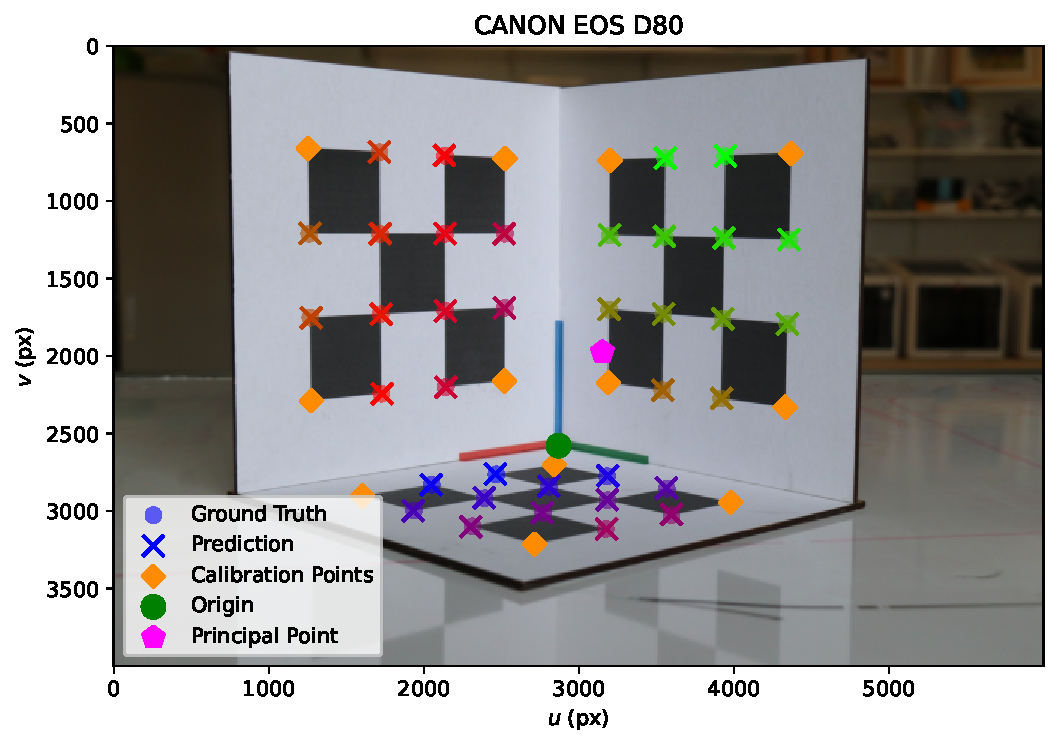
\includegraphics[width=0.75\textwidth]{assets/results/CANON EOS D80/graph.pdf}
        \caption{Canon EOS D80.}
    \end{subfigure}
    \begin{subfigure}{\textwidth}
        \centering
        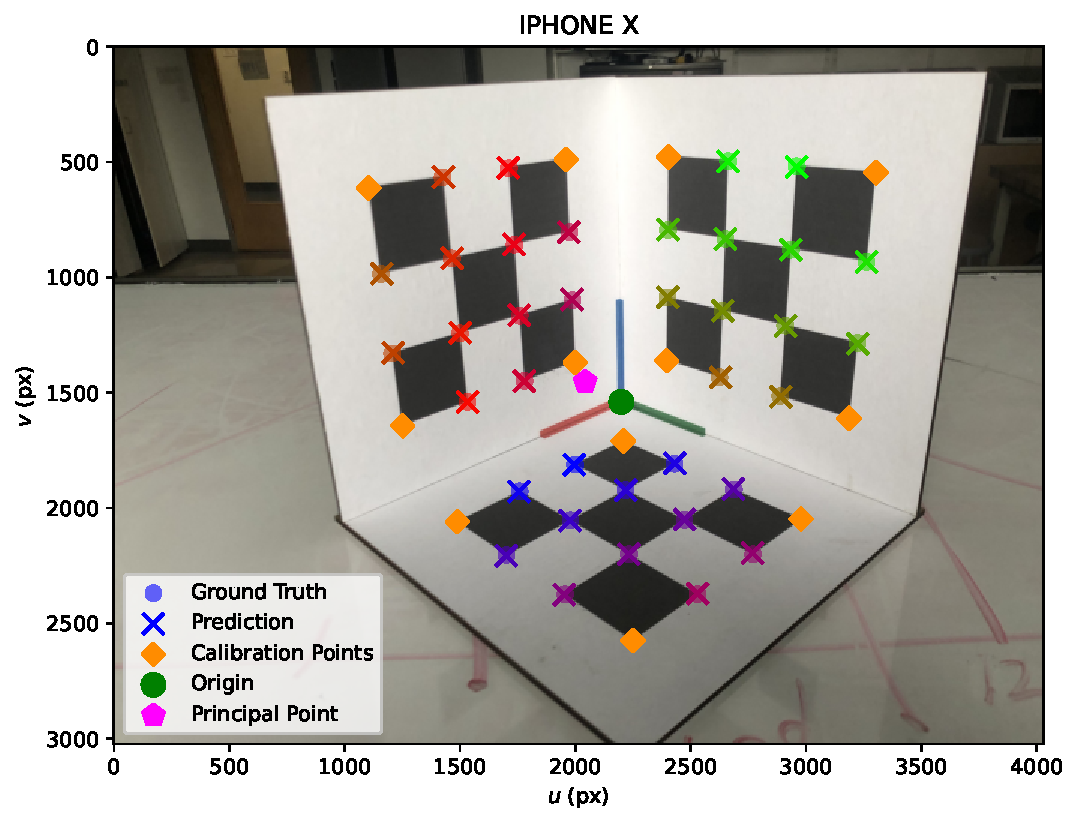
\includegraphics[width=0.75\textwidth]{assets/results/IPHONE X/graph.pdf}
        \caption{iPhone X.}
    \end{subfigure}
\end{figure}
\begin{figure}[H]
    \ContinuedFloat
    \centering
    \begin{subfigure}{\textwidth}
        \centering
        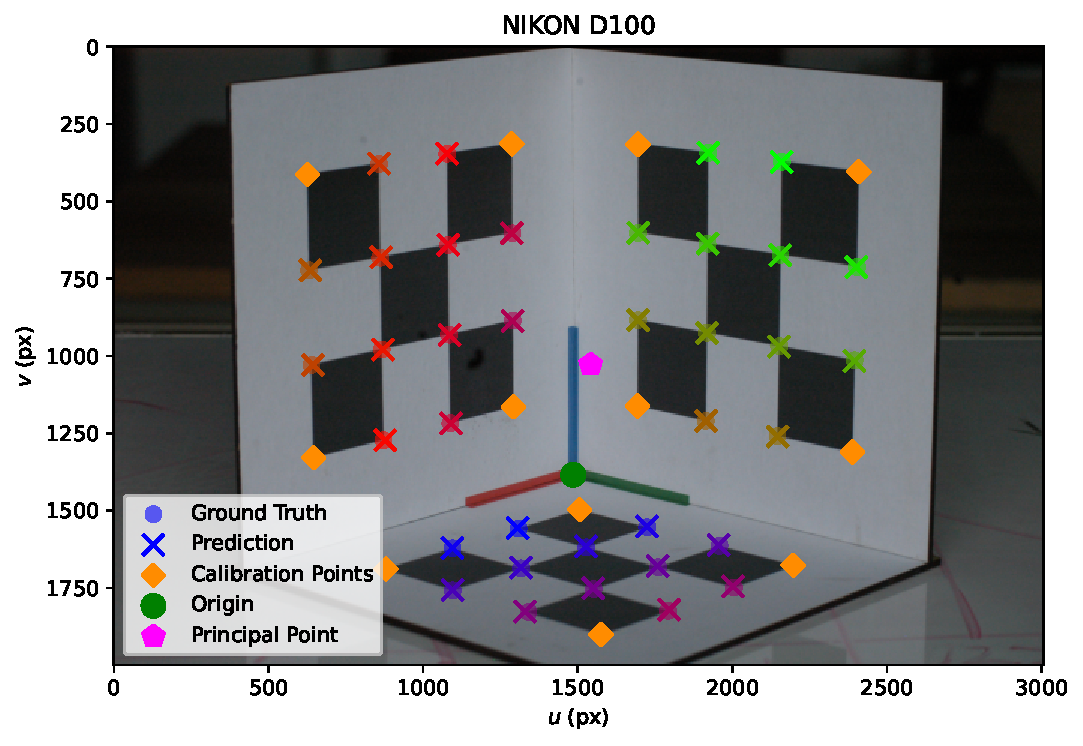
\includegraphics[width=0.75\textwidth]{assets/results/NIKON D100/graph.pdf}
        \caption{Nikon D100}
    \end{subfigure}
    \caption{Graphs generated by \texttt{calicam}.}
\end{figure}

\subsection{Validating Estimated Focal Length}
Given that specification of cameras are readily available online, we can actually further evaluate the accuracy of our model by calculating the focal lengths estimated by our model and comparing it to the manufacturer reported value. Assuming that the pixels are square, we estimate the focal lengths of our cameras to be the average of the horizontal and vertical focal lengths. Then, based on the manufacturer reported size of each individual pixel (known as the \emph{pixel pitch}), we can convert our estimated focal length from pixels to millimeters.

\begin{table}[H]
    \centering
    \resizebox{\columnwidth}{!}{
    \begin{tabular}{p{4.0cm}c@{\hskip 0.5cm}c@{\hskip 0.5cm}c}
        \toprule
                                      & \textbf{\small Calculated Focal Length}\tablefootnote{Pixel pitches retrieved from \url{digicamdb.com}.} & \textbf{\small Manufacturer Reported Focal Length} & \textbf{\small \% Error} \\
        \midrule
        \textbf{\small Canon EOS D80} & $(\qty{8496}{\pixel})(\qty{3.73e-3}{\milli\meter \per \pixel}) \approx \boxed{\qty{31.7}{\milli\meter}}$        & \qty{32}{\milli\meter}                & \qty{0.94}{\percent}     \\
        \textbf{\small IPhone X}      & $(\qty{3280}{\pixel})(\qty{1.22e-3}{\milli\meter \per \pixel}) \approx \boxed{\qty{4.00}{\milli\meter}}$        & \qty{4}{\milli\meter}                 & --                       \\
        \textbf{\small Nikon D100}    & $(\qty{8143}{\pixel})(\qty{7.82e-3}{\milli\meter \per \pixel}) \approx \boxed{\qty{63.7}{\milli\meter}}$        & \qty{55}{\milli\meter}                & \qty{15.6}{\percent}     \\
        \bottomrule
    \end{tabular}
}

    \caption{Comparison of Calculated vs. Reported Focal Length.}
\end{table}

Considering that the focal lengths reported by manufacturers are often only accurate to around $\pm \qty{1}{\milli\meter}$,\footcite{waynefAnswerAre2017} my results are very promising, with exception to the Nikon D100. However, this error is in fact a result of human error, as I forgot to turn off autofocus on the Nikon D100, and the zoom lens Nikon D100 altered the effective focal length.



\section{Conclusion}
Based on my initial experimental validation, it is evident that the camera calibration method which I have devised displays a high level of accuracy. Despite the lack of consideration of lens distortion by model, the results still displayed negligible reprojection errors. The method I devised was simple, as it only required a single image containing the calibration object, however, there are various weaknesses and downfalls to my method, most notably fixed focal length and limited adaptability to different localities, it serves as a proof of concept which excellently demonstrates the various strategies and mathematical techniques employed in camera calibration.


%TC:ignore
\section*{Acknowledgements}
\addcontentsline{toc}{section}{Acknowledgements}

I am very grateful to my EE supervisor for his continual guidance and invaluable pieces of advice during the process of writing this extended essay. Additionally, I would like to express my appreciation to Mr. Auclair for dedicating his time to instruct me on camera operation and familiarizing me with camera settings. I am also indebted to Leon, for his help in operating the laser cutter. Last but not least, I want to thank Aditya for helping me troubleshoot issues that came up when using Adobe Illustrator for creating diagrams used in my paper.

% =========================
\clearpage
\pagestyle{backmatter}
\printbibliography[heading=bibintoc]{}

\clearpage
\begin{appendices}
    \pagestyle{appendices}
    \clearpage
\section{Homogenous Coordinates} \label{sec:homogenous}

The standard Cartesian coordinate system has long served as the foundation for representing points and vectors in Euclidean space. However, certain limitations arise when dealing with transformations, particularly translations and perspective projections, both of which are operations core to this paper. To overcome these challenges, homogenous coordinates are employed.

\begin{definition}
    Given a point $(a_1, a_2, \cdots, a_n) \in \Real^n$, it can be expressed in homogenous coordinates as $(\lambda a_1, \lambda a_2, \cdots, \lambda a_n, \lambda) \in \Real^{n+1}$, where $\lambda \neq 0$ is a constant scale factor. 
\end{definition}

In other words, we essentially extend the coordinate representation to include an extra dimension

\begin{equation}
    \begin{bmatrix}
        u \\ v 
    \end{bmatrix}
    \sim
    \begin{bmatrix}
        u\widetilde{w} \\ v\widetilde{w} \\ \widetilde{w}
    \end{bmatrix}
    \equiv
    \begin{bmatrix}
        \widetilde{u} \\ \widetilde{v} \\ \widetilde{w}
    \end{bmatrix}
\end{equation}

One important property of homogenous coordinates is that if the homogenous coordinate of a point is multiplied by a non-zero scalar, the result represents the same point. i.e.
\begin{equation}
    \begin{bmatrix}
        \widetilde{u} \\ \widetilde{v} \\ \widetilde{w}
    \end{bmatrix}
    \equiv
    k
    \begin{bmatrix}
        \widetilde{u} \\ \widetilde{v} \\ \widetilde{w}
    \end{bmatrix}
    \qquad (k \neq 0)
\end{equation}

\begin{figure}[H]
    \centering
    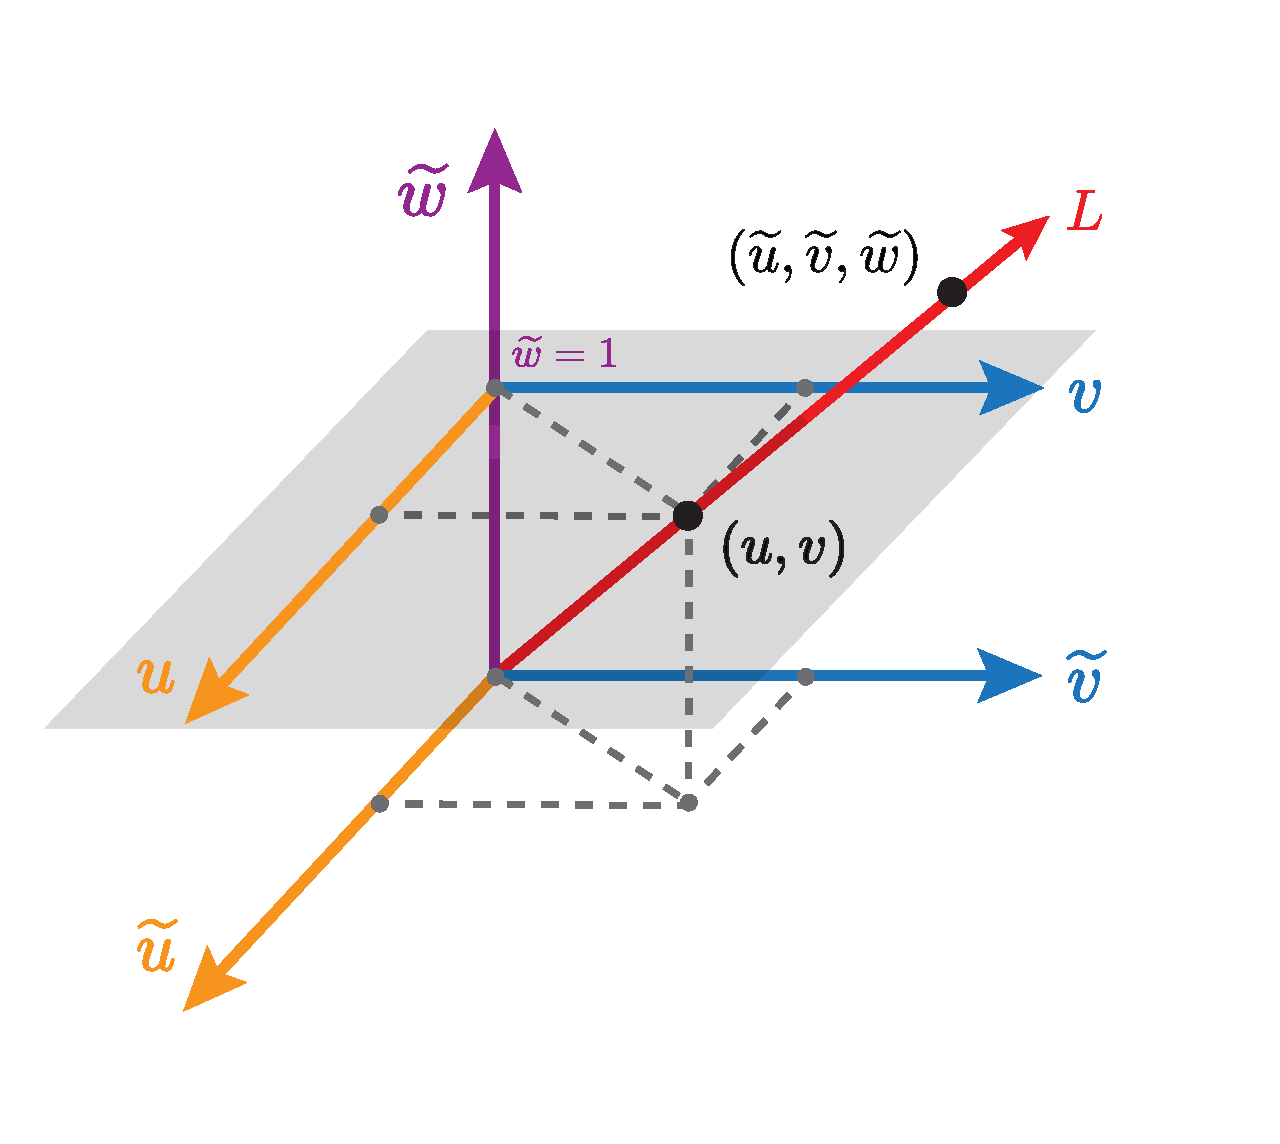
\includegraphics[width=0.6\textwidth]{diagrams/homogenous}
    \caption{Homogenous coordinate system.}
\end{figure}

    \section{Calibration Object Details}
\subsection{Panels}
\subsection{Grid Pattern}

\begin{center}
    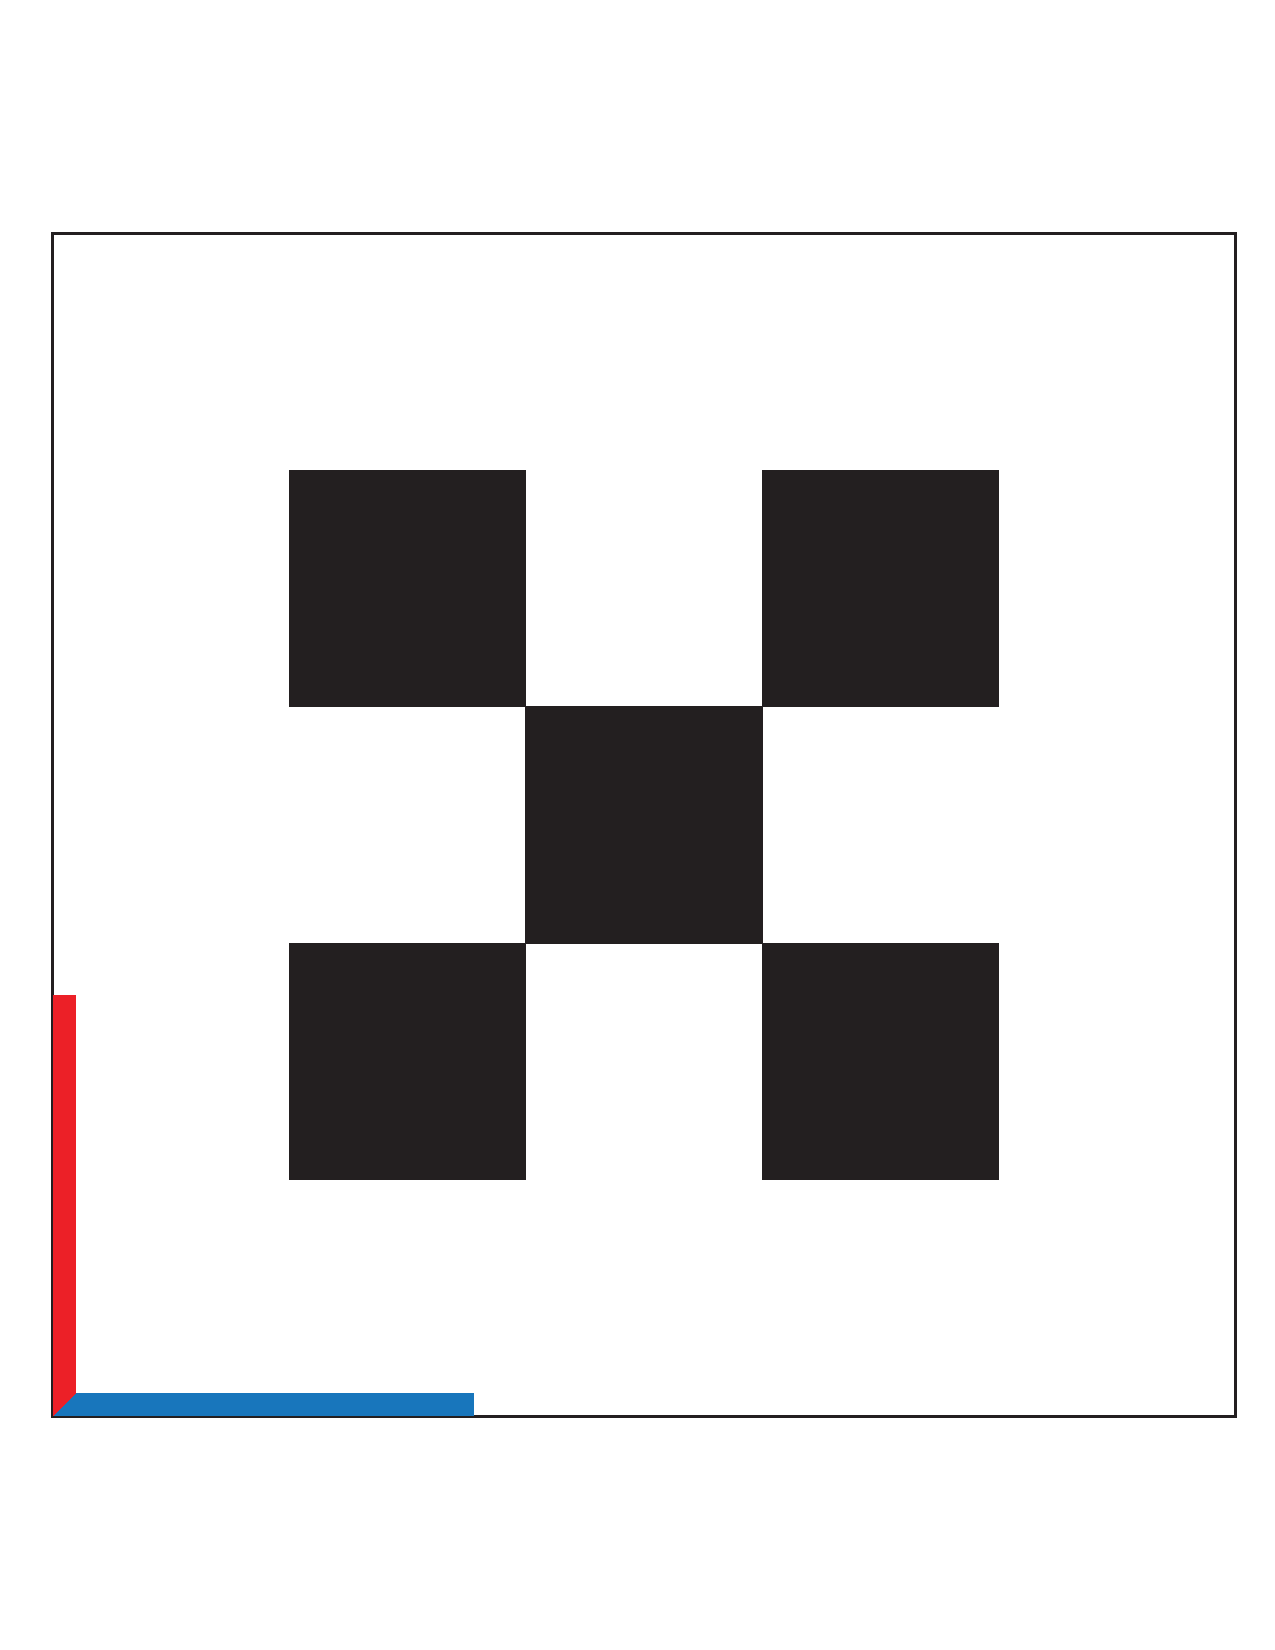
\includepdf[pages={1-}]{grid.pdf}
\end{center}


    \section{Source Code}

\subsection*{Project Structure}

\dirtree{%
    .1 calicam.
    .2 calicam.
    .3 \_\_init\_\_.py.
    .3 \hyperref[code:extract]{extract.py}.
    .3 \hyperref[code:parser]{parser.py}.
    .3 \hyperref[code:projection]{projection.py}.
    .3 \hyperref[code:vecs]{vecs.py}.
    .2 \hyperref[code:main]{main.py}.
}

\subsubsection*{main.py} \label{code:main}
\inputminted{python}{./calicam/main.py}

\subsubsection*{calicam/parser.py} \label{code:parser}
\inputminted{python}{./calicam/calicam/parser.py}

\subsubsection*{calicam/projection.py} \label{code:projection}
\inputminted{python}{./calicam/calicam/projection.py}

\subsubsection*{calicam/extract.py} \label{code:extract}
\inputminted{python}{./calicam/calicam/extract.py}

\subsubsection*{calicam/vecs.py} \label{code:vecsZ}
\inputminted{python}{./calicam/calicam/vecs.py}

\end{appendices}
%TC:endignore

\end{document} % END

